\documentclass[titlepage, 12pt]{article} 
\usepackage{verbatim}
\usepackage[T1]{fontenc}
\usepackage[utf8]{inputenc}
\usepackage[brazil]{babel}
\usepackage{hyperref}
\usepackage{rotating}
\usepackage{listings}
\usepackage{color}
\usepackage{float}
\usepackage{appendix}
\usepackage{amsmath, amsthm, amssymb}
\usepackage{multirow}
\usepackage{array}
\usepackage{geometry}
\usepackage{changepage}
\usepackage{lmodern}
\usepackage{scrextend}
\usepackage{enumitem}
\usepackage[none]{hyphenat}
\changefontsizes[14pt]{11pt}

\hypersetup{colorlinks=true,%
	citecolor=red,%
	linkcolor=red,%
	urlcolor=blue,%
	pdftex}

\definecolor{Brown}{cmyk}{0,0.81,1,0.60}
\definecolor{OliveGreen}{cmyk}{0.64,0,0.95,0.40}
\definecolor{CadetBlue}{cmyk}{0.62,0.57,0.23,0}

\newcommand{\opensource}{\textit{open source}}
\newcommand{\software}{\textit{software}}
\newcommand{\suricato}{Suricato}

\title{\suricato: Um sistema para facilitar reuniões de melhoria contínua}
\author{Lucas Takeshi Rodrigues Palma\\Márcio Sakamoto Shibao\\ \\Orientador: Prof. Dr. Alfredo Goldman\\Coorientadora: Cecilia Fernandes}

\begin{document}
	
\lstset{language=Java,frame=ltrb,framesep=5pt,basicstyle=\footnotesize,
  keywordstyle=\ttfamily\color{OliveGreen},
 identifierstyle=\ttfamily\color{CadetBlue}\bfseries, 
 commentstyle=\color{Brown},
 stringstyle=\ttfamily,
 showstringspaces=false,
 showspaces=false,
 tabsize=2}

\maketitle

\begin{abstract}
Seja em pequenos times de microempresas até times de times em contextos complexos, importantes processos de melhoria contínua acontecem a todo momento, nas mais diversas formas e nos mais diversos formatos. Em times de TI utilizando métodos ágeis, uma ferramenta bastante comum para promoção e efetivação dessas melhorias é a prática, em intervalos regulares, de retrospectivas.

Neste trabalho, analisamos a literatura ágil, explicando os passos recomendados para que times façam retrospectivas eficientes e eficazes. Em seguida, apresentamos uma revisão sistêmica sobre essas reuniões analisando primeiro o estado atual do uso de retrospectivas e, em segundo lugar, os diferentes tipos de estruturas de times e a distribuição dos mesmos no mundo ágil.

A terceira parte trata da pesquisa realizada na comunidade agil em busca de mais informações e dos resultados que indicam quais são as dificuldades enfrentadas por times ágeis na promoção de melhoria contínua. E, por fim, descrevemos os passos do planejamento e desenvolvimento de uma aplicação com base nos dados previamente adquiridos.


% No começo do trabalho foi preciso entender melhor sobre a retrospectiva. Este conhecimento foi adquirido após uma revisão sistemática do conceito. O próximo passo seria encontrar dados na comunidade que indicassem quais as necessidades que times ágeis enfrentam com retrospectiva.

% No entanto, poucos os artigos e pesquisas foram encontrados que tratavam do assunto. Assim, a ideia foi realizar uma pesquisa na comunidade ágil buscando obter dados sobre como está a adesão de retrospectivas pelos times, quais as dificuldades enfrentadas pelas equipes ao realizá-la e que outras práticas são usadas para promover a melhoria contínua. Após o término da pesquisa, houve uma análise das respostas obtidas para descobrir as necessidades das equipes.

% A partir desta analise, planejou-se uma aplicação cujos requisitos tinham como objetivo auxiliar as equipes nas dificuldades encontradas. Assim, começou o desenvolvimento do Suricato, um sistema que que serve como uma ferramenta para ajudar times ágeis a realizarem reuniões de melhoria continua. 
\end{abstract}
\newpage


\tableofcontents
\newpage

\begin{description} 
\item{\textbf{Alunos:}\\Lucas Takeshi Rodrigues Palma\\Márcio Sakamoto Shibao}
\item{\textbf{Supervisores:}\\Prof. Dr. Alfredo Goldman\\Cecilia Fernandes}
\item{\textbf{Colaboradores:}\\Fabio Gushiken\\Leonardo Guerra\\Marco Bruno\\Mauricio Aniche\\Alberto Tavares}
\end{description}

\section{Introdução}
Times ágeis são aqueles que seguem e otimizam os preceitos descritos no Manifesto Ágil~\cite{manifesto}. Esses times se preocupam em atender às expectativas do usuário, ainda que essas mudem no decorrer do projeto, além de melhorar a qualidade do trabalho executado pela equipe.

Um dos princípios definidos no manifesto discorre sobre a busca pela melhoria contínua das equipes:

\begin{quote}
	\textit{``At regular intervals, the team reflects on how to become more effective, then tunes and adjusts its behavior accordingly.''}~\cite{manifesto}
\end{quote}

 Para promover essa evolução, uma das práticas mais adotadas pelos times ágeis é a retrospectiva. Segundo Derby e Larsen~\cite{retrospectives}, retrospectiva é uma reunião especial em que o time se junta para investigar e melhorar seus métodos - um tempo dedicado à aprendizagem, que funciona como um catalisador de mudanças e ações. Em contraste às tradicionais lições aprendidas, ela foca tanto no processo de desenvolvimento, quanto nas questões humanas do projeto.

Desta forma, a retrospectiva cria um ambiente propício para pessoas ouvirem diferentes percepções e pontos de vista e, assim, ampliarem a visão sobre as diversas situações pelas quais o time passa. Essa reunião é, portanto, uma importante ferramenta, já que dá a oportunidade de entender como melhorar suas habilidades, a produtividade do time e a qualidade do produto para cada membro.

No entanto, por mais que os times ágeis conheçam a reunião e entendam seu funcionamento, a aplicação da teoria nem sempre apresenta bons resultados. Logo, o \suricato{} é um projeto que surgiu da ideia de ajudar times ágeis a realizarem retrospectivas com mais facilidade.

%TODO : revisar os parágrafos com a Ceci
A necessidade da aplicação surgiu na equipe em que ambos os idealizadores do projeto trabalham. Problemas como juntar todos os membros em um único dia, manter o foco das pessoas e organizar a reunião ocorriam de tempos em tempos e mesmo buscando e aplicando possíveis soluções, alguns desses problemas retornavam.

No entanto, a intenção do projeto não é substituir a retrospectiva presencial, mas prover uma ferramenta que  ajude os times ágeis a alcançarem a melhoria contínua. Além disso, o \suricato{} guarda históricos das reuniões para saber quais são as atividades realizadas com maior frequência pelos times e, eventualmente, sugerir para seus usuários novos formatos para a reunião.   

Esse texto está organizado da seguinte forma: na seção 2, explicamos a relação entre melhoria contínua e retrospectivas, assim como sua estrutura sugerida. Em seguida, na seção 3, descrevemos a pesquisa que foi submetida à comunidade ágil brasileira e os resultados obtidos. Na seção 4, explicamos o processo de construção do projeto Suricato, que visa auxiliar times a resolver os problemas levantados na pesquisa e, por fim, concluímos na seção 5 com nossos pareceres e expectativas para o futuro do projeto e da pesquisa.
\newpage

\section{Melhoria Contínua e Retrospectiva}

Com o passar do tempo, é comum que pessoas e times adotem certos padrões para conseguirem trabalhar juntos com menos atrito e de forma mais produtiva. No âmbito técnico, essa tendência se demonstra nas práticas de desenvolvimento utilizada. No pessoal, no formato da comunicação, sua frequência e relacionamento entre as pessoas envolvidas.

Como disse Aristóteles: 

\begin{quote}
\textit{``Só fazemos melhor aquilo que repetidamente insistimos em melhorar. A busca da excelência não deve ser um objetivo, e sim um hábito.''}
\end{quote}

Ou seja, sempre há espaço para melhorias. Assim, como não existe uma forma perfeita de se trabalhar, pessoas, processos e projetos devem estar em constante evolução.

No estudo de processos de desenvolvimento de projetos, outra literatura que trata melhoria contínua com grande seriedade é a \textit{Lean}: a filosofia por trás do modelo Toyota de produção~\cite{lean}. O conceito recebe o nome de \textit{Kaizen} e, em uma empresa que seguem as ideias do \textit{Lean}, todas as pessoas, independentemente de salário ou hierarquia, são responsáveis por pensar e agir para melhoria contínua do processo e do produto oferecido.

Esses são apenas alguns demonstrativos da importância do princípio de melhoria contínua: é interessante que os times usem parte do seu tempo para pensar no que está dando certo ou errado, quais áreas precisam de aperfeiçoamento e que ações podem ser tomadas para levar o time a uma evolução. Equipes que conseguem fazer isso, a longo prazo, aumentam a qualidade do código, entregam mais valor para o cliente e criam um ambiente de trabalho melhor, entre outros benefícios.

Aplicar os conceitos de melhoria contínua no dia a dia, contudo, não é uma tarefa trivial. Há diversas práticas e técnicas que podem servir para esse propósito e, no contexto dos métodos ágeis, a ferramenta mais conhecida com esse objetivo é a retrospectiva.

\subsection{Estrutura e papéis em retrospectivas}

Dependendo do contexto, uma retrospectiva pode se tornar uma reunião complexa, dividida em uma série de etapas e é comum que os participantes percam a visão do todo e se percam em algum problema. Assim, é interessante e muito comum que uma pessoa assuma um papel mais neutro, focando no andamento e nas atividades da reunião. Essa pessoa é chamada de \textbf{facilitador}.

Sua função é manter o time focado, sem dispersar durante discussões ou se alongar demais em temas pouco relevantes. Ele pode fazer isso, por exemplo, relembrando o assunto principal, delimitando tempos máximos para cada assunto, ou estruturando as atividades que comporão a reunião.

Durante a retrospectiva, o time deve ser capaz de identificar obstáculos e situações adversas. Esse é o momento para identificar problemas, definir ações e responsáveis por fazer cada ação ser cumprida e, assim, tornar todo o time responsável por fazer melhorias acontecerem.

Para organizar tudo isso, há diversas publicações sugerindo formatos para essa reunião. O formato apresentado por Derby e Larsen~\cite{retrospectives} no livro Agile Retrospectives é o mais conhecido entre agilistas:

\begin{enumerate}
	\item Preparar o terreno: 5\% do tempo.
	\item Coletar os dados: 30\% a 50\% do tempo.
	\item Gerar ideias: 20\% a 30\% do tempo.
	\item Decidir o que fazer: 15\% a 20\% do tempo.
	\item Encerrar a retrospectiva: 10\% do tempo.
\end{enumerate}

Para realizar a retrospectiva com essas 5 etapas, o facilitador pode inventar atividades que façam esse papel, ou se valer de diversas técnicas já catalogadas em páginas da internet ou livros, tais quais \textit{Fun Retrospectives}~\cite{funRetrospectives}, \textit{Retrospective Handbook}~\cite{handRetrospectives} e \textit{Agile Retrospectives}~\cite{retrospectives}.

\subsubsection*{Preparar o terreno}

O objetivo desta etapa é ajudar o time a se concentrar no que será feito no decorrer da reunião e passar para os participantes qual será o objetivo da retrospectiva.

Além disso, é nesta etapa que se estabelece o ambiente no qual as pessoas discutirão. Para garantir que a reunião focará na melhoria do time, é necessário garantir que cada pessoa se sinta confortável para expressar suas opiniões e contribuir com as discussões.

\subsubsection*{Coletar os dados}

Mesmo com iterações curtas, tipicamente de uma ou duas semanas, e times pequenos, de até dez pessoas, é improvável que todos tenham conhecimento e participação em tudo que aconteceu com o time.

Antes de decidir o que fazer, é importante que todos criem uma visão uniforme sobre o que aconteceu no projeto recentemente, levando em conta as opiniões e pontos de vista de cada pessoa do time. A etapa de coleta de dados busca expor as opiniões e visões de cada membro do time para estabelecer uma mesma imagem dos acontecimentos que estão em discussão.

Existem dois tipos de dados a serem coletados: fatos e aspectos subjetivos. Os fatos, são eventos, métricas, funcionalidades, histórias terminadas, e demais itens tangíveis. A análise destes pode ajudar as pessoas a encontrar padrões e fazer ligações entre os últimos acontecimentos. Os dados subjetivos, são as impressões, opiniões, julgamentos de importância e valor que cada integrantes atribui aos fatos.

O levantamento dessas informações, baseados em ambos os tipos de dados apresentados, leva a uma visão maior sobre o que está correndo bem e o que precisa de ações para melhoria.

\subsubsection*{Gerar ideias}

Depois que um ambiente propício para discussões é estabelecido e todos estão olhando para os mesmo dados, é o momento de dar um passo pra trás para visualizar a imagem que foi gerada e pensar no que fazer. 

Esta é a etapa em que as pessoas investigam quais foram os problemas enfrentados, quais vitórias alcançaram e os riscos a que projeto e time estão suscetíveis. A partir destas discussões, todos os membros do time propõem diversas ações sobre o que pode ser feito em busca de melhorias.

A fase de gerar ideias pode ser executada de forma orgânica, quando todos os membros se sentirem confortáveis em lançar ideias livremente, ou de forma mais estruturada e impessoal, quando a equipe ainda não está madura. Técnicas como \textit{brainstorming} e \textit{brainwriting}~\cite{brainwriting}, termos utilizados em inglês mesmo na literatura brasileira sobre o tema, são bastante comuns nessa fase.

\subsubsection*{Decidir o que fazer}

Após obter um conjunto de ideias, chega o momento de selecionar as mais promissoras, transformá-las em ações e escolher aquelas que o time se compromete a executar.

Como as ideias vieram de todos, é comum que as pessoas apontem muitas ações e queiram adotar todas. No entanto, a literatura e especialistas em agilidade indicam índices melhores de sucesso na execução das ações de retrospectivas quando o time se compromete com um número pequeno delas, preferindo as de melhor relação custo-benefício.

Além disso, é interessante delegar a alguém a responsabilidade por realizar a ação planejada -- quando ninguém fica como responsável é bem comum que a mudança não seja feita.

Ao final da fase de decidir o que fazer, portanto, temos um pequeno conjunto de ações que buscam promover melhorias, já atribuidas a indivíduos ou sub-grupos que ficarão responsáveis pelo seu cumprimento.

\subsubsection*{Encerrar a retrospectiva}

No decorrer da retrospectiva o time esteve, a todo momento, discutindo e propondo ideias. Embora nem todas as ideias que foram apresentadas sejam selecionadas, existe valor no simples fato de todos terem tido sua chance de expor o que observaram e como se sentiram. Essa reunião cria, naturalmente, um maior senso de time. Para manter tal sensação, é comum que o facilitador separe um tempo para lembrar ao time desse fato.

Além disso, o facilitador pode buscar os pontos positivos e negativos sobre a própria reunião promovendo, dessa forma, uma breve retrospectiva da retrospectiva. Assim, haverá \textit{feedback} para que a próxima reunião seja ainda melhor conduzida e a escolha de atividades também se adeque mais às preferências do time para a próxima vez.

\subsection{Ferramentas usadas em retrospectivas}

Uma forma utilizada para realizar a retrospectiva é usando uma lousa para apresentar a atividade da reunião e post-its para coletar os dados. Este processo funciona para times cujos membros trabalham no mesmo local. Para as equipes em que as pessoas estão distribuídas em diferentes regiões, existem ferramentas que simulam a estrutura da reunião local.

A Retrium~\footnote{https://retrium.com/} oferece um serviço web para times realizarem a reunião seguindo uma estrutura próxima da apresentada por Derby e Larsen~\cite{retrospectives}. Ele começa com a escolha de uma atividade, seguido da coleta dos dados, agrupamento de informações comuns, priorização dos comentários mais relevantes e termina com a geração das ideias.

O principal problema da aplicação é o baixo número de atividades oferecidas. Atualmente ela suporta apenas 3 formatos conhecidos de retrospectiva:

\begin{itemize}
	\item Mad, Sad and Glad
	\item Start, Stop and Continue
	\item Liked, Learned, Lacked and Longed for
\end{itemize}

Todos estes formatos seguem o princípio de discutir apenas os problemas da equipe, ignorando retrospectivas que discutem, por exemplo, o futuro ou a cultura do time. 

Outro problema é a falta de flexibilidade do sistema que exige que o usuário siga o mesmo fluxo para a reunião. Usuários que já estão acostumados com o processo da retrospectiva costumam adaptar a reunião para o seu cenário, o que não é possível fazer através da Retrium.

A GroupMap~\footnote{http://www.groupmap.com/map-templates/agile-retrospective/} oferece um serviço que trabalha apenas com as atividades mais simples, que verificam apenas os pontos positivos e negativos. Os problemas são bem parecidos com os encontrados na Retrium, como a falta de flexibilidade no fluxo da reunião. Os times não habituados com a retrospectiva também podem achar o sistema complexo, uma vez que não há marcações ou dicas sobre o que são cada um dos recursos.

Essas aplicações focam apenas na realização da retrospectiva e atinge apenas os times que já sabem realizá-la. No entanto, existem problemas que não são cobertos por essas aplicações.
\newpage

\section{Pesquisa}

Tanto a melhoria contínua quanto a retrospectiva já são conceitos muito conhecidos e utilizados pela comunidade ágil. Como cada time possui suas próprias necessidades e dificuldades, é comum a equipe adaptar estes conceitos para a sua situação. Isto dificulta para encontrar informações sobre como a melhoria contínua é aplicada atualmente e saber quais são as dificuldades que os times ágeis enfrentam ao realizar estas reuniões, principalmente a retrospectiva. 

Alguns destes dados só foram obtidos a partir de uma revisão sistemática da literatura sobre retrospectivas e quais são os problemas em seu desenvolvimento. No entanto, a maior parte do material que existe hoje foca na aplicação da reunião e nos passos durante a retrospectiva.

Os artigos que mostram o estado atual dos times ágeis consistem em relatórios de questionários que indicam a quantidade de times que fazem retrospectivas, como as pesquisas da VersionOne~\cite{versionOne} e da Scrum Alliance~\cite{scrumAlliance}. Em geral, os relatórios mostram a porcentagem de times que estão em cada etapa da adoção dos métodos ágeis, desde a introdução dessas metodologias na equipe até sua total adequação. Eles também mostram dados como a distribuição demográfica dos times que adotaram agilidade e quais métricas as equipes utilizam.

Boa parte das pesquisas apontavam que o uso de retrospectivas vem constantemente aumentando nos últimos anos. No entanto, são poucos os trabalhos que apresentam as dificuldades enfrentadas pelos times e, em geral, o assunto é tratado apenas para equipes locais. Existem duas possibilidades para essa falta de informação sobre equipes remotas: times usarem outras formas de promover melhoria contínua ou não haver publicações sobre o tema na comunidade.

Devido a falta de material de apoio para levantar estas informações, foi feita uma pesquisa sobre as práticas utilizadas por times locais e distribuídos, e quais desafios eles enfrentavam.

Para abranger uma parte ainda maior da comunidade ágil e enviesar menos o questionário em relação à ferramenta usada para trazer o princípio da melhoria contínua à tona, o assunto da pesquisa seria não apenas retrospectivas, mas o tópico maior: como times ágeis promovem melhoria de forma contínua.

\subsection{Motivação e questões da pesquisa}

Considerando, então, que o tema da pesquisa é o princípio de melhoria contínua, as questões foram imparciais de modo a não direcionar as respostas em torno apenas das retrospectivas. A parte inicial foca em questões gerais, como o número de integrantes, a distribuição da equipe e quais os desafios enfrentados. Depois são investigadas as particularidades sobre qual prática cada time utiliza para solucionar esses problemas e promover a melhoria contínua. 

Como a retrospectiva ainda é utilizada por diversos métodos ágeis e muitos times, parte do questionário é voltado apenas para as equipes que realizam esta reunião. As questões desta etapa buscam encontrar como cada time estrutura a reunião, quais os principais problemas que as equipes enfrentam na retrospectiva e a relação deles com a estrutura de cada time. 

Além disso, os artigos encontrados previamente já indicam que, embora nem todos os times façam a retrospectiva, eles ainda adotam alguma outra forma de promover a melhoria contínua. A última parte da pesquisa foca justamente nesses times que utilizam práticas diferentes da retrospectiva. Para estes casos, o questionário procura quais são as outras opções que são adotadas, como é o processo para realizar cada uma e os motivos que levaram o time a usar uma prática diferente da retrospectiva.

\subsection{Resultados}

O tempo para a coleta de respostas foi de 1 mês e foram obtidas 44 respostas. A pesquisa era composta de respostas quantitativas, com o intuito de coletar os problemas enfrentados e a utilização de retrospectivas, e qualitativas, que buscavam entender como os times resolviam seus problemas.

\subsubsection*{Resultados das perguntas quantitativas}

A primeira parte da pesquisa indicou que diferentes estruturas de equipes apontam diferentes problemas. A separação foi feita em: 
  
\begin{itemize}
  \item Local: times que estão no mesmo ambiente
  \item Distribuído no mesmo \textit{timezone}: times que não estão no mesmo ambiente, mas no mesmo fuso horário.
  \item Distribuído em \textit{timezones} diversos: times que não estão no mesmo ambiente e estão distribuídos em diferentes fusos horários.
\end{itemize}

Em seguida, são identificados os problemas que cada uma das equipes enfrentam, como, por exemplo, comunicação, relacionamento e produtividade. Como cada uma das estruturas possui as suas singularidades, os desafios enfrentados potencialmente estão relacionados com a distribuição dos integrantes. A análise desses dois dados em conjunto segue na tabela abaixo.

\begin{table}[H]
  \begin{adjustwidth}{-3em}{}
    \begin{tabular}{  m{6em}  m{3em} | m{6em} | m{7em} | m{6em} | m{5em} | m{5em} | }
      \cline{3-7} & & \multicolumn{5}{ c| }{Quais problemas seu time enfrenta? } \\ 
      \cline{1-7} \multicolumn{1}{ |m{6em}| }{Estrutura majoritária do time} & Total & Comunicação & Relacionamento & Produtividade & Nenhum & Outros \\
      \cline{1-7} \multicolumn{1}{ |m{6em}| }{Local} & 27 & 15 (55\%) & 4 (14\%) & 18 (66\%) & 4 (14\%) & 2 (7\%) \\ 
      \cline{1-7} \multicolumn{1}{ |m{6em}| }{Distribuído no mesmo \textit{timezone}} & 11 & 5 (45\%) & 1 (9\%) & 4 (36\%) & 3 (27\%) & 1 (9\%) \\
      \cline{1-7} \multicolumn{1}{ |m{6em}| }{Distribuído em \textit{timezones} diversos} & 6 & 4 (66\%) & 2 (33\%) & 1 (16\%) & 0 (0\%) & 3 (50\%) \\
      \cline{1-7} \multicolumn{1}{ |m{6em}| }{Total} & 44 & 24 (54\%) & 7 (15\%) & 23 (52\%) & 7 (15\%) & 6 (13\%) \\
      \cline{1-7}
    \end{tabular}
  \end{adjustwidth}
\end{table}

O desafio mais enfrentado por times ágeis é a comunicação. A pesquisa mostra que aproximadamente 54\% das equipes passam por esse problema. Além disso, os times distribuídos em \textit{timezones} diversos tendem a sofrer mais com este problema, já que 66\% deles passam por esta dificuldade, enquanto que os percentuais dos locais e distribuídos no mesmo \textit{timezone} foram de 55\% e 45\%, respectivamente.
  
Outro desafio no qual os times distribuídos em diversos fusos horários aparentam ter mais dificuldades do que as outras equipes é a de relacionamento. Aproximadamente 33\% dessas equipes relataram que passam por esse problema, contra apenas 14\% dos locais e 9\% dos distribuídos no mesmo \textit{timezone}.
  
Apesar dos times distribuídos em diversos fusos terem mais problemas de comunicação e relacionamento, eles possuem o melhor rendimento entre as três estruturas. Apenas 16\% deles possuem problemas de produtividade. Já para os times distribuídos no mesmo \textit{timezone} o valor chegou a 36\%, ou seja, mais do que o dobro. Porém, os times que mais sofrem com este problema são os locais que apresentaram um percentual de 66\%.
  
Por fim, os times distribuídos em \textit{timezones} diversos apresentaram outros problemas que não foram apontados pelas outras estruturas. A pesquisa mostrou que eles tem dificuldade para sincronizar todos os seus membros. Como as pessoas trabalham em fusos horários diferentes fica difícil definir as datas para os diversos tipos de reuniões ágeis, como o \textit{daily}, o \textit{planning}, a \textit{review} e a retrospectiva.

Após as questões sobre os desafios que cada um dos tipos de times ágeis enfrentam, os próximos resultados mostram como esses problemas são resolvidos e de que forma a melhoria contínua é promovida. Diversas pesquisas e artigos da área indicam que a grande maioria das equipes adotam a retrospectiva como uma das práticas ágeis utilizadas. A pesquisa apenas confirmou essa hipótese e mostrou como é sua aceitação pelos diversos tipos de equipes.

\begin{table}[H]
  \centering
  \begin{tabular}{  m{6em}  m{3em} | m{6em} | m{7em} |}
    \cline{3-4} & & \multicolumn{2}{ c| }{Seu time realiza retrospectivas?} \\ 
    \cline{1-4} \multicolumn{1}{ |m{6em}| }{Estrutura majoritária do time} & Total & Sim & Não \\
    \cline{1-4} \multicolumn{1}{ |m{6em}| }{Local} & 27 & 21 (77\%) & 6 (22\%) \\
    \cline{1-4} \multicolumn{1}{ |m{6em}| }{Distribuído no mesmo \textit{timezone}} & 11 & 9 (81\%) & 2 (18\%) \\
    \cline{1-4} \multicolumn{1}{ |m{6em}| }{Distribuído em \textit{timezones} diversos} & 6 & 1 (16\%) & 5 (83\%) \\
    \cline{1-4} \multicolumn{1}{ |m{6em}| }{Total} & 44 & 31 (70\%) & 13 (29\%) \\
    \cline{1-4}
  \end{tabular}
\end{table}

Aproximadamente 70\% dos participantes responderam que realizam retrospectivas. No entanto, é interessante notar como foram as respostas para cada uma das estruturas das equipes. Os times locais e distribuídos no mesmo \textit{timezone} são os que mais utilizam desta reunião como prática de melhoria contínua. Em contrapartida, aqueles que são distribuídos em \textit{timezones} diversos não costumam realizar retrospectivas já que apenas 16\% responderam que sim.

Um questão que ainda não foi comprovada pelos artigos na comunidade é se a retrospectiva realmente auxilia os times a resolver seus problemas. A pesquisa mostrou os seguintes resultados. 

\begin{table}[H]
  \begin{adjustwidth}{-3em}{}
    \begin{tabular}{ m{6em} m{3em} | m{6em} | m{7em} | m{6em} | m{5em} | m{5em} | }
      \cline{3-7} & & \multicolumn{5}{ c| }{Quais problemas seu time enfrenta?} \\ 
      \cline{1-7} \multicolumn{1}{ |m{6em}| }{Seu time realiza retrospectiva?} & Total & Comunicação & Relacionamento & Produtividade & Nenhum & Outros \\
      \cline{1-7} \multicolumn{1}{ |m{6em}| }{Sim} & 31 & 16 (51\%) & 3 (9\%) & 17 (54\%) & 6 (19\%) & 3 (9\%) \\
      \cline{1-7} \multicolumn{1}{ |m{6em}| }{Não} & 13 & 8 (61\%) & 4 (30\%) & 6 (46\%) & 1 (7\%) & 3 (23\%) \\
      \cline{1-7} \multicolumn{1}{ |m{6em}| }{Total} & 44 & 24 (54\%) & 7 (15\%) & 23 (52\%) & 7 (15\%) & 6 (13\%) \\
      \cline{1-7}
    \end{tabular}
  \end{adjustwidth}
\end{table}

Os resultados mostram que a retrospectiva ajuda os times ágeis. Entre os que não realizam retrospectiva, o percentual de problemas foi de 61\% para comunicação e 30\% para relacionamento, respectivamente. Já para os times que a utilizam os percentuais foram de 51\% e 9\%. Além disso, aqueles que não usam desta prática aparentam ter problemas mais diversos dos que os que fazem, pois 9\% daqueles que responderam que sim assinalaram a opção outros, enquanto que para aqueles que responderam não o percentual de 23\%.
    
Outro fator que mostra que retrospectivas auxiliam os times a evoluir foram os resultados na opção "Nenhum". Apenas 7\% dos times que não usam esta prática ágil assinalaram esta opção, enquanto que entre os que a utilizam apresentaram um resultado de 19\%. Isso pode ser um indicativo de potenciais problemas no time já que, como visto antes, é suspeito que um time simplesmente não tenha problema algum -- é mais provável que os problemas existam, mas que o time não esteja ciente deles.

Um resultado que contraria a perspectiva inicial é a produtividade. Os times que não realizam retrospectivas apresentaram melhores resultados neste quesito, já que o seu percentual foi de 46\%, contra 54\% dos que fazem a reunião. Este fato pode ocorrer por conta da maior parte dos times que responderam não estão classificados na categoria times distribuídos em \textit{timezones} diversos. Como apresentado acima, estes times são os que mostraram os melhores resultados em termos de produtividade, o que pode ter influenciado o resultado mostrado acima.

Conclui-se que as retrospectivas têm de fato auxiliado os times no processo de melhoria contínua. Porém, ainda há espaço para ajudar as equipes nesta reunião.

Os próximos resultados mostram os principais desafios que os times enfrentam durante a retrospectiva.

\begin{table}[H]
  \begin{adjustwidth}{-4em}{}
    \begin{tabular}{  m{3em} | m{5.5em} | m{5em} | m{5em} | m{5em} | m{5.5em} | m{5em} | m{5em} | }
      \cline{2-8} & \multicolumn{7}{ c| }{Quais desafios seu time enfrenta ao realizar uma retrospectiva?} \\ 
      \cline{1-8} \multicolumn{1}{ |m{3em}| }{Total} & Ultrapassar a duração & Agendar dia, horário e lugar & Discussões de pouco valor & Falta de intimidade entre integrantes & Engajamento das pessoas & Falta de anonimato & Outros \\
      \cline{1-8} \multicolumn{1}{ |m{3em}| }{19} & 10 (52\%) & 1 (5\%) & 8 (42\%) & 4 (21\%) & 9 (47\%) & 1 (5\%) & 3 (15\%) \\
      \cline{1-8}
    \end{tabular}
  \end{adjustwidth}
\end{table}

A pesquisa apontou que os principais desafios enfrentados pelos times ágeis são ultrapassar a duração, falta de engajamento das pessoas e discussões de pouco valor. Uma hipótese levantada por alguns artigos, como Poussard~\cite{poussard},  é que os times sofrem com a falta de engajamento e as discussões de pouco valor por conta deles não variarem as atividades que utilizam nas retrospectivas. Através da pesquisa é possível verificar esta suspeita através da correlação entre os desafios com o fato do time variar ou não as atividades. Os resultados desta análise estão a seguir.

\begin{table}[H]
  \small
  \begin{adjustwidth}{-6.5em}{}
    \begin{tabular}{ m{5.5em} m{3em} | m{5em} | m{5em} | m{5em} | m{5em} | m{5.5em} | m{5em} | m{5em} | }
      \cline{3-9} & & \multicolumn{7}{ c| }{Quais desafios seu time enfrenta ao realizar uma retrospectiva?} \\ 
      \cline{1-9} \multicolumn{1}{ |m{5.5em}| }{Você varia as atividades e/ou formato das suas retrospectivas?} & Total & Ultrapassar a duração & Agendar dia, horário e lugar & Discussões de pouco valor & Falta de intimidade entre integrantes & Engajamento das pessoas & Falta de anonimato & Outros \\
      \cline{1-9} \multicolumn{1}{ |m{5.5em}| }{Sim} & 8 & 4 (50\%) & 0 (0\%) & 3 (37\%) & 1 (12\%) & 4 (50\%) & 1 (12\%) & 2 (25\%) \\
      \cline{1-9} \multicolumn{1}{ |m{5.5em}| }{Não} & 11 & 6 (54\%) & 1 (9\%) & 5 (45\%) & 3 (27\%) & 5 (45\%) & 0 (0\%) & 1 (9\%) \\
      \cline{1-9}
    \end{tabular}
  \end{adjustwidth}
\end{table}

Os resultados mostram que os percentuais dos problemas são próximos entre aqueles que variam ou não as atividades. Porém, alguns deles confirmaram as expectativas, como o fato de que equipes que não variam as retrospectivas têm mais problemas de discussões de pouco valor. Estes times tiveram um percentual de 45\% para este desafio, enquanto para aqueles que variam seus formatos de retrospectiva o resultado foi de 37\%.

Além disso, os times que variam suas atividades aparentam sofrer menos com falta de intimidade entre integrantes em relação às equipes que não variam, pois os resultados foram de 12\% e 27\%, respectivamente.

Para a falta de engajamento das pessoas as porcentagens foram muito próximas e os times que responderam que não variam tiveram um melhor resultado, contrariando as expectativas. Então não ficou evidente que alternar os formatos de retrospectiva ajuda os times com todos os desafios.

Apesar da pesquisa apontar que somente alternar as atividades não é suficiente, incentivar os times a variar os formatos de retrospectiva que eles utilizam pode ajudá-los a enfrentar alguns dos desafios desta reunião.

Uma outra forma conhecida para diminuir os problemas em uma retrospectiva é o uso do facilitador. A correlação entre a quantidade de desafios com o uso ou não do facilitador é apresentada na próxima tabela.

\begin{table}[H]
  \small
  \begin{adjustwidth}{-6.5em}{}
    \begin{tabular}{ m{5.5em} m{3em} | m{5em} | m{5em} | m{5em} | m{5em} | m{5.5em} | m{5em} | m{5em} | }
      \cline{3-9} & & \multicolumn{7}{c|}{Quais desafios seu time enfrenta ao realizar uma retrospectiva?} \\ 
      \cline{1-9} \multicolumn{1}{ |m{5.5em}| }{Alguém fica responsável por facilitar as retrospectivas?} & Total & Ultrapassar a duração & Agendar dia, horário e lugar & Discussões de pouco valor & Falta de intimidade entre integrantes & Engajamento das pessoas & Falta de anonimato & Outros \\
      \cline{1-9} \multicolumn{1}{ |m{5.5em}| }{Sim} & 17 & 8 (47\%) & 1 (5\%) & 8 (47\%) & 4 (23\%) & 9 (52\%) & 1 (5\%) & 3 (17\%) \\
      \cline{1-9} \multicolumn{1}{ |m{5.5em}| }{Não} & 2 & 2 (100\%) & 0 (0\%) & 0 (0\%) & 0 (0\%) & 0 (0\%) & 0 (0\%) & 0 (0\%) \\
      \cline{1-9}
    \end{tabular}
  \end{adjustwidth}
\end{table}

O questionário mostrou que é quase unânime o uso do facilitador nas retrospectivas. São 17 dos 19 times que responderam a pesquisa que usam deste recurso, o que corresponde a 89\% das equipes.
    
Como apenas dois times responderam que não têm um facilitador responsável por suas reuniões, não é possível encontrar padrões de desvio entre o grupo maior e esse par de respostas. Porém, nota-se que ambas as equipes que responderam ''Não'' reportaram problemas em ultrapassar a duração da reunião -- é possível que o uso desta técnica ajude no melhor controle do tempo.

Mesmo usando o facilitador, aproximadamente metade dos times tem problemas como ultrapassar a duração (47\%), discussões de pouco valor (47\%) e falta de engajamento das pessoas (52\%). Logo, somente com uma pessoa facilitando a reunião não garante que as retrospectivas serão bem-feitas.

\subsubsection*{Resultados das perguntas qualitativas}

Para complementar as informações obtidas com as respostas quantitativas, a pesquisa também possui questões qualitativas que se relacionam com os dados anteriores. 

Uma das perguntas busca investigar o porquê do baixo número de equipes geograficamente distribuídas fazendo retrospectiva. Como os resultados anteriores demonstram problemas de sincronização nestes times, um motivo para eles não realizarem retrospectivas é devido à impossibilidade de reunir todos os membros para a discussão em algum horário. Além disso, alguns artigos encontrados pressupõem que somente os gerentes e líderes de projeto participavam das discussões e decidiam o que seria feito.

Duas respostas apontaram que a razão para o time não realizar a retrospectiva é devido a falta de tempo, já que ambos alegaram que a equipe está passando por período de alta demanda. Outros dois participantes responderam que o motivo vem a partir de uma decisão dos gestores do projeto. Uma dessas respostas também revelou que o gerente não possui experiência com metodologias ágeis. Além disso, um outro participante também indicou que não é cultura da empresa utilizar desta prática. 

Somente com estas informações não é possível tirar conclusões definitivas sobre o porquê deles não realizarem retrospectivas. Uma hipótese é que esses times ainda não possuem experiência suficiente com métodos ágeis e também não dispõem de pessoas engajadas em agilidade que queiram aplicar retrospectivas como forma de inspecionar problemas. Logo, eles acabam não vendo o valor dessa reunião e o retorno que ela proporciona. Essa hipótese é reforçada a partir das respostas sobre como os problemas nesses times são discutidos e resolvidos, quem participa das discussões e quem aplica as mudanças para solucionar o problema.

Os times que responderam anteriormente que não fazem retrospectivas devido a alta demanda indicaram que realizam \textit{conference calls} entre os membros do time para debater sobre os problemas do time. Em geral, essas reuniões não tem um horário previsto para acontecer e todos os integrantes participam. Percebe-se, assim, uma inconsistência nas respostas destes participantes, pois ambos alegam que o time não possui tempo para realizar a retrospectiva, mas eles conseguem mobilizar todos os membros para uma reunião onde serão discutidos os problemas. Desta forma, torna-se mais provável que a razão pela qual eles não utilizam a retrospectiva é pela falta de experiência com agilidade, não conhecer a fundo esta prática e saber o valor que esta reunião pode proporcionar.

Da mesma forma, também houve inconsistências nas respostas dos outros times que apontaram que a razão para não realizarem a reunião é por conta de uma decisão dos gestores ou por não ser parte da cultura da empresa. Estes times conversam via chat para discutir os seus problemas e todos os membros que possuem disponibilidade participam ativamente do debate. Caso as pessoas encontrem uma solução interessante para o problema, ela é informada para o restante da equipe e para o gerente do projeto. 

Logo, a forma como esses times promovem melhoria contínua é muito semelhante à retrospectiva. Provavelmente a única diferença é que algumas das atividades utilizadas em retrospectivas motivam o time a conversar sobre o futuro. Nas respostas que os participantes deram quando questionados de que forma o time identifica os problemas futuros e trabalha para evitá-los, a grande maioria indicou que a equipe não tem esse tipo de preocupação. Apenas um participante comentou que os integrantes passam por essa discussão, mas focada apenas no código da aplicação. Ou seja, eles não possuem uma preocupação em debater sobre o futuro do projeto e do time.

Como nenhum dos participantes mencionou o nome de alguma prática de melhoria contínua, como o \textit{Kaizen} ou \textit{Hansei}, não é possível concluir se estas reuniões são baseadas em algum outro tipo de prática ágil diferente da retrospectiva. Além disso, nota-se que as decisões não são tomadas somente pelos gerentes, \textit{coachs} e líderes de projeto, mas sim por todos os integrantes da equipe. Desta forma, não existem grandes impeditivos para mesmo os times distribuídos realizarem suas reuniões seguindo os preceitos da retrospectiva. Um sistema que auxilie essas equipes a sincronizarem seus horários e forneça uma plataforma para realizar essas reuniões estruturadas pode motivar os times a usarem a retrospectiva como prática de melhoria contínua.

\subsection{Conclusão}

A pesquisa forneceu dados importantes que não eram encontrados em publicações na comunidade. Por exemplo, as informações de quais estruturas de times usam a retrospectiva, que dificuldades estas equipes enfrentam na reunião e que outras formas de melhoria contínua são adotadas por aqueles que não fazem a retrospectiva.

Sem a pesquisa, não é possível ter uma ideia da realidade atual que os diversos times ágeis estão enfrentando e que ainda há muitas dificuldades para serem superadas. 

Saber as reais necessidades dos times ágeis é vital para planejar uma estratégia de como auxiliá-los. Pensando nisso, foi possível planejar uma aplicação focada em melhoria contínua, usando como base os resultados obtidos a partir da pesquisa.
\newpage

\section{Desenvolvimento}

A partir dos resultados obtidos na pesquisa o próximo passo do trabalho foi  planejar e desenvolver um sistema com o objetivo de auxiliar os times ágeis nas suas reuniões de melhoria contínua.

O levantamento dos requisitos foi feito em meados de agosto e a implementação da aplicação ocorreu de setembro até novembro. O código do projeto está em um repositório do GitHub~\footnote{https://github.com/mxball/suricato}.

\subsection{Planejamento}

O planejamento da aplicação ocorreu de meados de agosto até o começo de setembro. Como o objetivo da aplicação é ajudar qualquer tipo de equipe, seja local ou distribuído, uma das necessidades é que a aplicação seja acessível pelas máquinas de todos os integrante, independente de sistema operacional. Portanto a opção foi desenvolver uma aplicação web, já que o usuário consegue acessar o sistema através de qualquer navegador.

\subsection{Requisitos do sistema}

A próxima etapa do trabalho foi levantar quais seriam os requisitos do sistema web e usando como base os resultados da pesquisa sobre os desafios que times ágeis enfrentam com reuniões de melhoria contínua.

A primeira coisa levada em consideração foi que a grande maioria dos times ainda fazem retrospectivas, com exceção dos times distribuídos em diversos fusos horários. A pesquisa mostrou que esses times ainda fazem reuniões parecidas com a retrospectiva, como, por exemplo, as conference calls. A única diferença é que elas não seguem uma estrutura como a retrospectiva, como a apresentada por Derby e Larsen~\cite{retrospectives}. Desta forma, decidiu-se basear os requisitos da aplicação na forma como a retrospectiva é feita localmente, mas a aplicação não exige que o time siga o fluxo predefinido pelas retrospectivas, como outras aplicações encontradas no mercado fazem, como, por exemplo, a retrium~\footnote{https://retrium.com/}.

\subsubsection*{Lousa virtual}

Em geral, a forma como as retrospectivas são feitas por times locais é utilizando um quadro branco, post-its e canetas. No começo da reunião o facilitador apresenta no quadro algum formato de retrospectiva, também conhecido como atividade. Depois de explicar a atividade para as pessoas, cada integrante pode colocar na lousa post-its, dando suas opiniões, apontando problemas no time, entre outros. A partir dos post-its o time consegue discutir e gerar ideias sobre como melhorar. Cada uma das ideias são escritas na lousa ou em post-its. Por fim, o time escolhe as melhores e define ações que o serão adotadas pela equipe para implementá-la. Essas ações também podem ser escritas na lousa ou em post-its.

Portanto o primeiro requisito definido foi que o usuário da aplicação pode criar uma lousa virtual. Ele escolhe um formato de retrospectiva e o sistema gera uma tela como um quadro branco com a atividade escolhida desenhada no fundo.

Depois de criar a lousa virtual, a próxima funcionalidade foi que o usuário poderia adicionar post-its. A tela daria algumas opções de post-its com diferentes cores e o integrante do time escreve algum texto no post-it depois de colocá-lo no quadro. Além da adição, outros dois requisitos definidos foram a remoção e edição.

Para representar a parte de escrever as ideias e ações, a ideia do projeto é que o usuário também adicione comentários na lousa. Da mesma forma que o post-it, a pessoa também consegue remover e editar um comentário.

\subsubsection*{Falta de engajamento e discussões de pouco valor}

Dois desafios muito citados pelos times que fazem a retrospectiva foram a falta de engajamento das pessoas e as discussões são de pouco valor. Poussard~\cite{poussard} aponta que um dos costumes que times ágeis tem é que muitos acabam criando hábitos nas retrospectivas e executando sempre os mesmos tipos de atividades. Ele defende que isso acaba enfraquecendo a evolução que poderia ser conquistada. Segundo Derby e Larsen~\cite{retrospectives},  as pessoas tendem a perder o interesse na retrospectiva quando estão fazendo sempre as mesmas atividades.

Para investigar se os pontos levantados nesses artigos, na pesquisa havia uma pergunta para times que fazem retrospectiva se eles alternam os tipos das suas atividades e, caso sim, quais são as atividades. Depois de correlacionar essa resposta com a pergunta sobre os desafios que eles enfrentam com a reunião, a pesquisa foi inconclusiva já que os resultados para cada uma das dificuldades entre aqueles que variam e os que não variam foram muito próximos.

Analisando as respostas é possível que os times variem as atividades, mas não os tipos de atividades. Das retrospectivas citadas pelos times que responderam sim, a maior parte delas eram do formato de encontrar problemas e discutir soluções. A hipótese é que muitos times ágeis ainda não conhecem diversos tipos de retrospectiva, como, por exemplo, as Futurespectives. Desta forma, eles alternam de atividade e não de tipo, como Pussard defende.

Como a pesquisa não foi suficiente para contrapor os artigos, decidiu-se por planejar alguns requisitos que incentivam os usuários a variar seus tipos de atividades. Para isso, o sistema deveria conter uma listagem com os mais diversos formatos de atividades para o usuário escolher. A hipótese é que apresentando as diversas opções pode ajudar os times a conhecer novas retrospectivas e alternar entre os diversos tipos. Isso pode ajudar os times com seus problemas de falta de engajamento das pessoas e as discussões pouco produtivas.

\subsubsection*{Tempo real}

Como os times são formados por um conjunto de pessoas e como elas podem estar espalhados por diversas regiões, um dos principais requisitos definidos é que todos os integrantes devem mexer na mesma lousa virtual. As lousas foram planejadas  para funcionarem em tempo real para muitos usuários, ou seja, todos os usuários estão visualizando a mesma lousa e tudo que for alterado por alguma pessoa será mostrado no navegador dos outros integrantes.

\subsubsection*{Dot voting (votação nas opções preferidas)}

Outra dificuldade que foi muito citada na pesquisa é ultrapassar a duração da reunião. Uma das causas desse problema é que durante a coleta dos dados, como cada integrante vai adicionar os seus post-its, a quantidade de dados acaba sendo muito grande. Muitas equipes decidem discutir todos os pontos levantados e acabam estourando o tempo definido para a reunião.

Na retrospectiva, uma das formas de reduzir o número de post-its que serão discutidos é encontrar quais são os pontos mais relevantes para se discutir. Para isso cada integrante vota nos pot-its que ele considera mais importantes e somente os mais votados serão discutidos na reunião. Essa forma de filtrar os dados é conhecida nas retrospectivas como dot votes.

Por se tratar de uma técnica eficiente de diminuir o tempo da reunião e influenciar o time a debater o que é mais essencial, foi decidido que o sistema deve possibilitar essa votação. Mesmo sendo um recurso específico da retrospectiva, ele pode ajudar inclusive os times que realizam outras reuniões de melhoria contínua. Desta forma, o último requisito definido para a primeira versão do projeto é que o usuário pode dar up votes em um post-it. Cada um dos votos que o post-it recebe é marcado na tela, assim os integrantes podem indicar quais são os mais relevantes.

\subsection{Trello}

Para organizar os requisitos e todos os participantes do projeto saberem o que estava sendo implementado, um dos sistemas usados para gerenciar o trabalho foi o Trello. Para cada um dos requisitos são criados cartões que definem o que será implementado.

\begin{figure}[H]
  \hspace*{-4em}
  \fbox{
    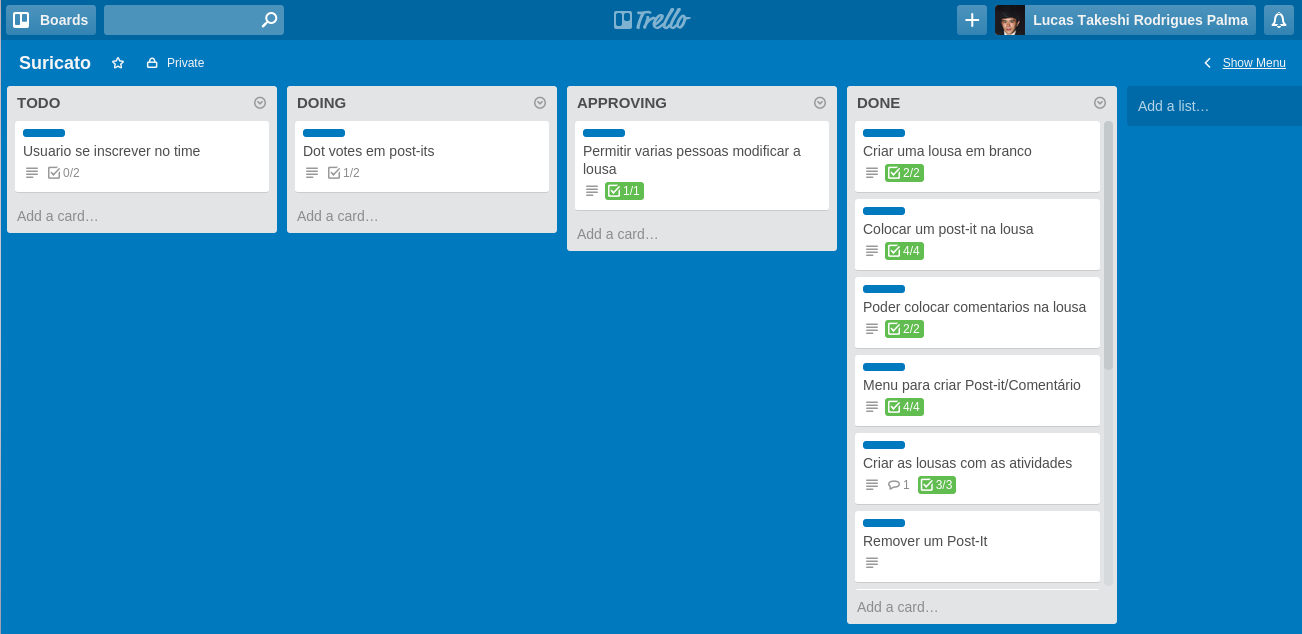
\includegraphics[width=170mm]{images/requisitos.png}
  }
  \caption{Requisitos do sistema}\label{figura:requisitos}
\end{figure}

Cada um desses cartões segue os modelos de cartões de história da agilidade, em que são dadas três informações:

\begin{itemize}
	\item Para: por que é importante que o sistema tenha essa funcionalidade
	\item Como: que tipo de usuário se beneficia mais com essa funcionalidade
	\item Quero: objetivamente, o que se quer que o software faça
\end{itemize}

\begin{figure}[H]
  \hspace*{-4em}
  \fbox{
    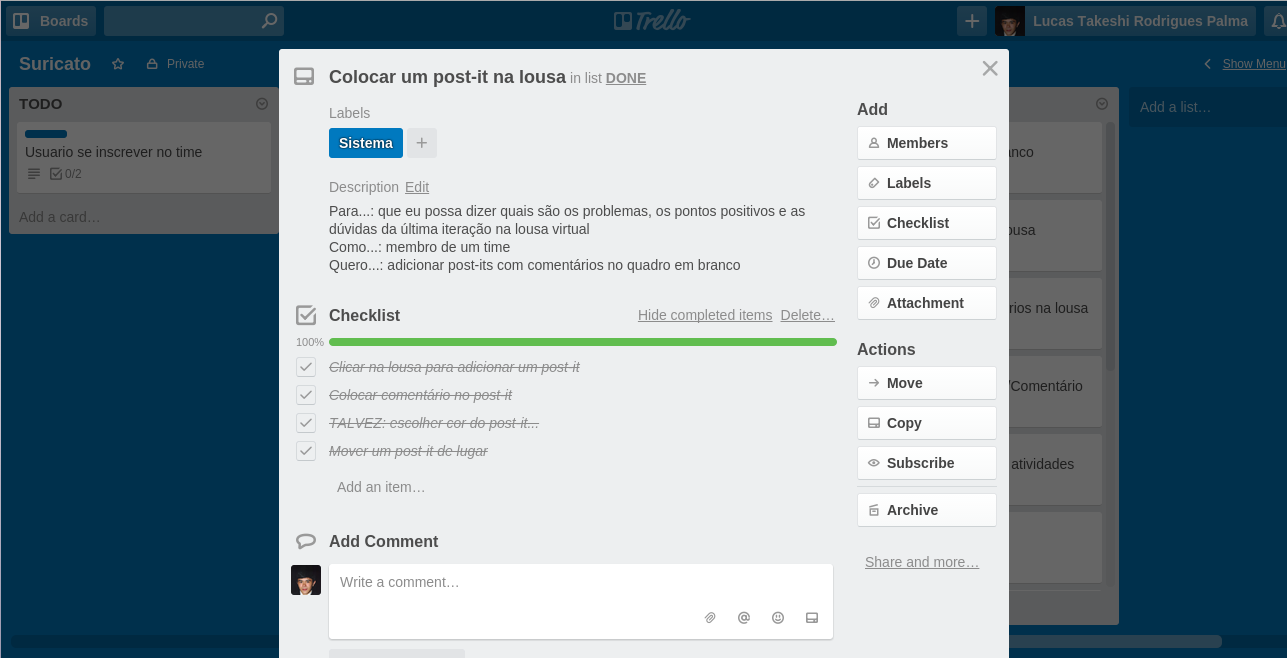
\includegraphics[width=170mm]{images/cartaoHistoria.png}
  }
  \caption{Modelo de cartão de história}\label{figura:cartao}
\end{figure}

\subsection{Tecnologias e criação do projeto}

O desenvolvimento da aplicação começou em setembro após o levantamento dos requisitos. Devido a familiaridade dos idealizadores do trabalho, a linguagem escolhida foi o Java. Ainda houve uma discussão sobre que tecnologias utilizar para desenvolver o sistema.

\subsubsection*{Framework MVC}

Hoje em dia, uma das formas mais utilizadas no mercado para desenvolver aplicações web é através da arquitetura MVC (Model View Controller), na qual seu sistema é dividido em três partes:

\begin{itemize}
	\item Models: classes que representam as entidades do sistema (por exemplo, usuário e time) e as que te ajudam a armazenar e buscar os dados.
	\item Views: responsável por apresentar os resultados na página web.
	\item Controllers: responsável por processar as requisições, instanciar os modelos necessários para realizar a tarefa requisitada e chamar as views.
\end{itemize}

Existem diversos frameworks no mercado que seguem essa estrutura e o escolhido para desenvolver o TCC foi o Spring MVC.

\subsubsection*{Autenticação e Autorização}

Como um dos requisitos do sistema era que uma pessoa pode criar uma lousa virtual e todos os integrantes do seu time participam da reunião através da mesma lousa, uma das necessidades do sistema é que o usuário precisa se identificar através de um login (autenticação) e quando ele tentar acessar alguma tela o sistema precisa verificar se ele possui permissão (autorização).

Já existem diversos frameworks no mercado que já abstraem as lógicas de autenticação e autorização, sendo necessário apenas informar qual o modelo de usuário usado pelo sistema. O framework escolhido foi o Spring Security devido a facilidade de integração com o Spring MVC.

\subsubsection*{Banco de dados}

Desde o início do projeto era óbvio que a aplicação precisaria de alguma banco para guardar os seus dados, como, por exemplo, os usuários, lousas virtuais, entre outros. A base de dados usada é o MySQL.

O sistema ainda precisava se integrar com o banco para conseguir armazenar o seus dados. O sistema está escrito na linguagem Java, cujo paradigma é a Orientação a Objetos. Desta forma, todos os modelos são representados através de classes e objetos. No entanto, os bancos de dados como MySQL que seguem o paradigma Relacional, ou seja, tudo é guardado em tabelas. Por representarem os dados de formas completamente diferentes, existe uma barreira de comunicação entre a aplicação e o banco.

Já existem diversos frameworks no mercado que já abstraem essa comunicação entre o aplicações orientadas a objetos e bancos relacionais, conhecidos como ORM (Object-relational Mapping). O mais utilizado é o Hibernate e foi a escolha para o projeto.

\subsubsection*{Servidor de aplicação e WebSockets}

Por se tratar de uma aplicação web, é essencial escolher em qual servidor rodará o sistema. Como um dos requisitos do sistema era que as lousas pudessem ser acessadas por vários usuários e as alterações deveriam ser em tempo real. Uma das formas conhecidas para fazer essa funcionalidade é usando o conceito de WebSockets. Ele é um protocolo de redes que estabelece como criar um canal de comunicação entre o navegador e o servidor.

Através dos WebSockets, toda vez que um usuário acessar uma lousa virtual é criado um canal com o servidor, conhecido como socket. Através delel o navegador consegue enviar mensagens para o servidor informando todas as ações feitas pelo usuário, como adicionar um post-it, editar um comentário, entre outros. Quando o servidor receber essa mensagem ele consegue armazena no banco essa informação e a retransmite para todos os sockets que ele possui. Desta forma, cada integrante que está acessando a lousa virtual recebe a mensagem através do socket informando alguma alteração feita por outra pessoa e consegue reproduzí-la na sua tela.

Essa ferramenta dos WebSockets ainda é recente e não são todos os servidores de aplicação que possuem suporte nativo para esse protocolo. Por isso o servidor escolhido foi o WildFly, desenvolvido pela RedHat, que já possui suporte para o WebSockets.

\subsubsection*{Nascimento do Suricato}

Uma das partes mais complicadas no começo de um grande projeto web é a integração entres os diversos frameworks que serão usados. Isso envolve muitas horas escrevendo diversos arquivos de configuração, em geral arquivos XML (Extensible Markup Language). Mesmo programadores com mais experiência levam longas horas até que todas as configurações fiquem corretas. 
	
No caso deste trabalho a integração seria entre os frameworks Spring MVC, Spring Security e Hibernate. Para não ocupar muito tempo com a configuração, o projeto foi gerado através do site Setup My Project~\footnote{http://www.setupmyproject.com/}. Ele permite que uma pessoa escolha quais tecnologias seu projeto usará e gera automaticamente uma versão simples de um sistema com todos os frameworks escolhidos já configurados.

Criando o projeto no Setup My Project, bastou colocá-lo para rodar no servidor WildFly para ter um ambiente configurado e começar a implementar os requisitos do sistema em meados de setembro.

Bastava dar um nome para o projeto. Devido uma antiga tradição no IME de que os projetos são do instituto recebem o nome de animais, a inspiração veio de procurar algum animal que saiba trabalhar bem em equipe. Assim o sistema do Suricato nasceu.

\subsubsection*{Dificuldades de integração WildFly WebSockets e Spring MVC}

Mesmo com o frameworks configurados, ainda faltava habilitar o WebSocket implementado pelo WildFly para funcionar com o Spring MVC, o que acabou gerando alguns problemas na hora de implementar o sistema para funcionar em tempo real.

A classe criada no sistema responsável por criar e utilizar o WebSocket do lado do servidor é a RetrospectivaEndpoint. Para marcá-la como uma classe do WebSocket basta anotar a classe com um @ServerEndpoint e passar qual a url pela qual o canal de comunicação será criado.

O problema aconteceu para conseguir armazenar as informações no banco de dados. Todos os códigos usados para comunicação com o banco foram isolados em classes que seguem o padrão de projeto DAO~\footnote{http://www.oracle.com/technetwork/java/dataaccessobject-138824.html}. Por trabalhar com o framework do Spring MVC, as classes DAO são anotadas com o @Repository. Com esta anotação, quem passa a gerenciar a classe -- cria objetos a partir dela e distribui esses objetos para outras classes que precisam usá-la -- é o Spring MVC. Esta forma de trabalhar do framework segue dois padrões de projeto, o Inversion of Control Containers e a Dependency Injection~\footnote{http://www.martinfowler.com/articles/injection.html}.

Então o cenário do sistema é que havia a classe RetrospectivaEndpoint, gerenciada pelo servidor de aplicação WildFly. Esta classe precisava receber objetos DAO's para enviar as informações para o banco de dados, mas estes são gerenciados pelo framework Spring MVC. O problema é que as duas tecnologias não são capazes de enviar objetos que uma delas está gerenciando para a outra automaticamente.

Mesmo pesquisando em blogs e fóruns se outras pessoas já passaram por esse problema de integração e como elas resolveram, nenhuma informação foi encontrada. Depois de algum tempo estudando mais a fundo as tecnologias e com a ajuda de pessoas da Caelum surgiu uma forma resolver este problema. O Spring MVC possui uma classe chamada de ApplicationContext, que possui objetos de todas as classes que ele gerencia, como os DAO's. Bastava criar a classe auxiliar ApplicationContextHolder, gerenciado pelo Spring e que possui um atributo estático que guarda um objeto de ApplicationContext. Por ser estático, qualquer outra classe do projeto pode acessá-lo, independente de qual tecnologia a gerencia. Assim, a classe RetrospectivaEndpoint consegue receber uma instância de ApplicationContext e, consequentemente, ao DAO.

Esta solução para o problema de integrar o WebSockets do servidor de aplicação WildFly com o framework Spring MVC foi publicado no blog sobre Spring de um colega da Caelum~\footnote{https://domineospring.wordpress.com/2015/11/03/um-pouco-de-gambi-nao-faz-mal-a-ninguem-spring-em-ambientes-nao-gerenciados/}. 

\subsection{Testes do software}

Depois de um mês de desenvolvimento, o sistema já tinha as funcionalidades mínimos para que alguma pessoa pudesse usá-lo. Um usuário conseguia criar a lousa, escolher entre diversas atividades para a reunião e adicionar, remover ou editar um post-it ou comentário. Faltava adicionar a autenticação e autorização, deixar a lousa funcionando em tempo real e os dot votes.

Como já era um sistema utilizável, os idealizadores do projeto começaram a usá-lo para fazer as retrospectivas do time em que trabalham. Com isso, diversos testes das funcionalidades foram feitos, o que permitiu encontrar alguns bugs e definir novas funcionalidades para o sistema.

Dentre as novas funcionalidades definidas depois de realizar os testes, as principais foram:

\begin{enumerate}
	\item o usuário pode regular o tamanho de um comentário e o tamanho dos post-its é fixo.
	\item comentários sempre aparecem por cima de um post-it.
	\item no campo de texto que deve ser preenchido ao criar o post-it ou comentário, a tecla Enter insere o elemento na tela e o Shift + Enter pula uma linha.
\end{enumerate}

\subsubsection*{Layout}

Em meados de novembro todas as funcionalidades já estavam implementados. No entanto, um dos pontos que mais discutidos durante os testes foi o layout do Suricato. Como os idealizadores do projeto ainda não possuem muita experiência na área de design e user experience, todas as telas do sistema continham pouco estilo e não eram muito agradáveis visualmente.

\begin{figure}[H]
  \centering
  \fbox{
    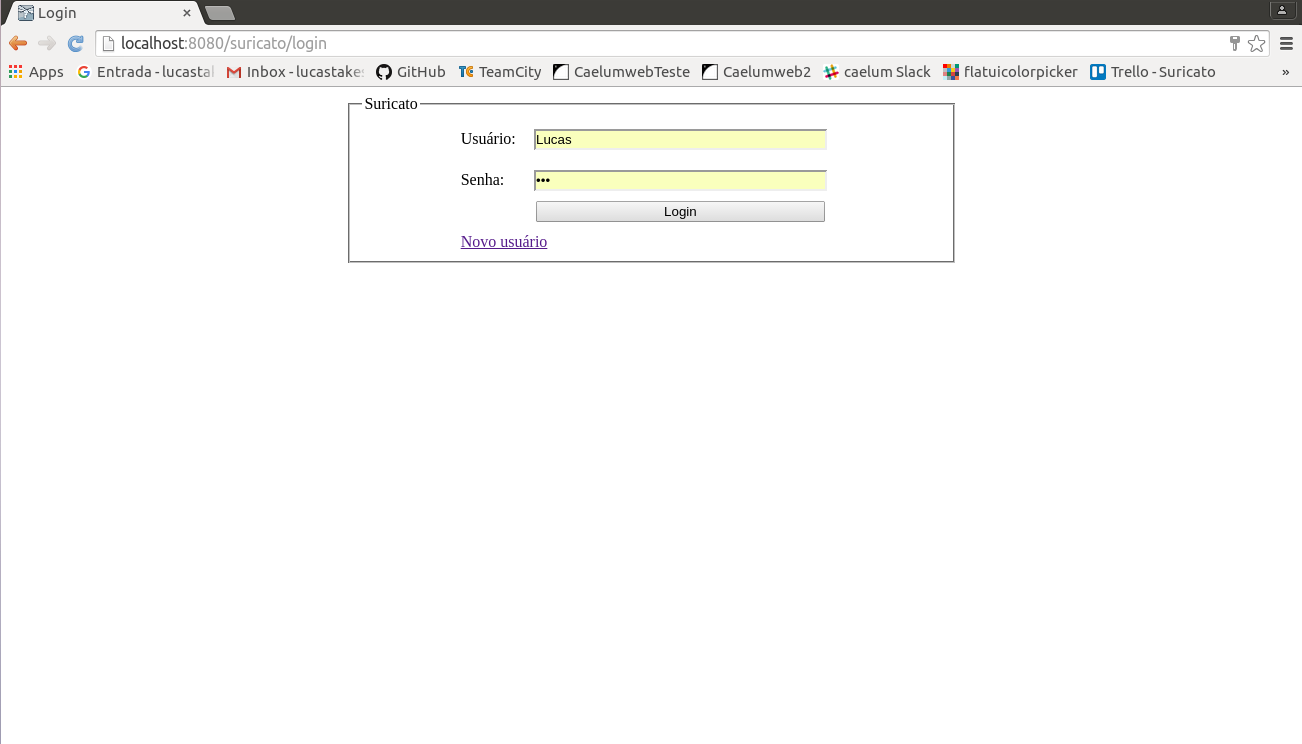
\includegraphics[width=130mm]{images/login.png}
  }
  \caption{Tela antiga de login}\label{figura:loginAntigo}
\end{figure}

\begin{figure}[H]
  \centering
  \fbox{
    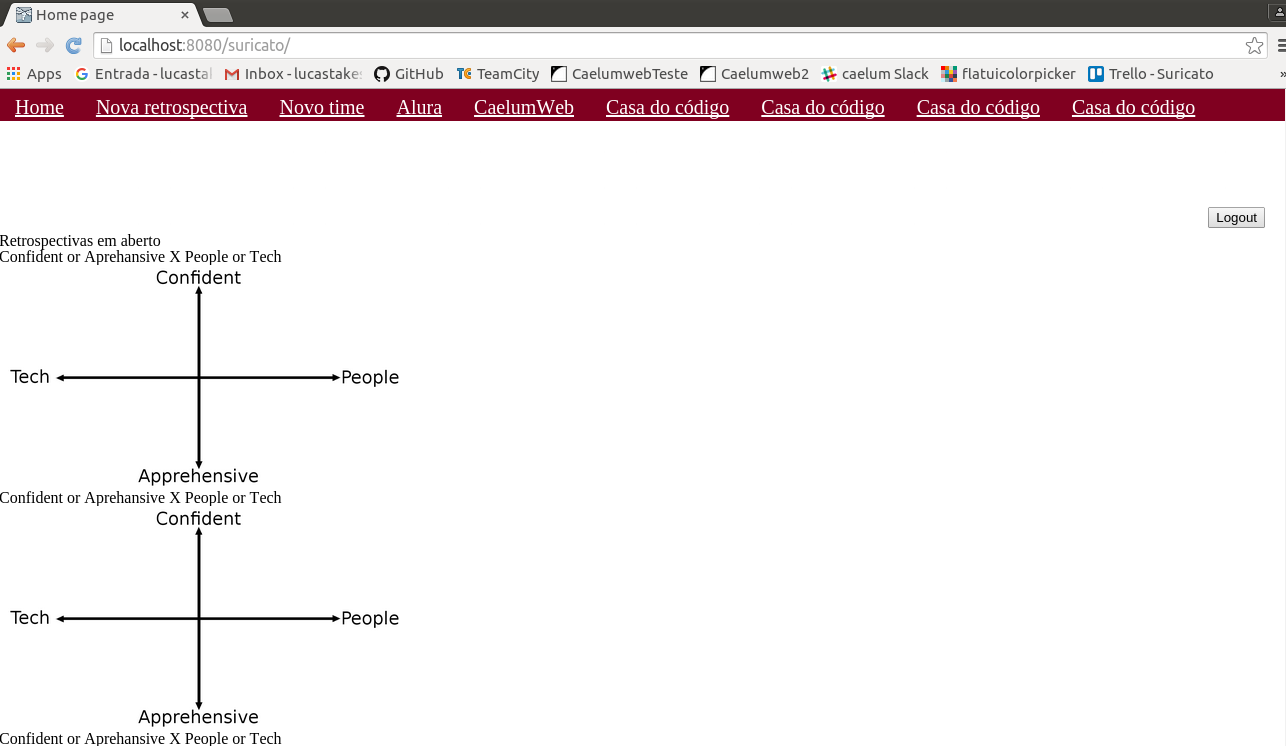
\includegraphics[width=130mm]{images/index.png}
  }
  \caption{Tela antiga do usuário}\label{figura:indexAntigo}
\end{figure}

\begin{figure}[H]
  \centering
  \fbox{
    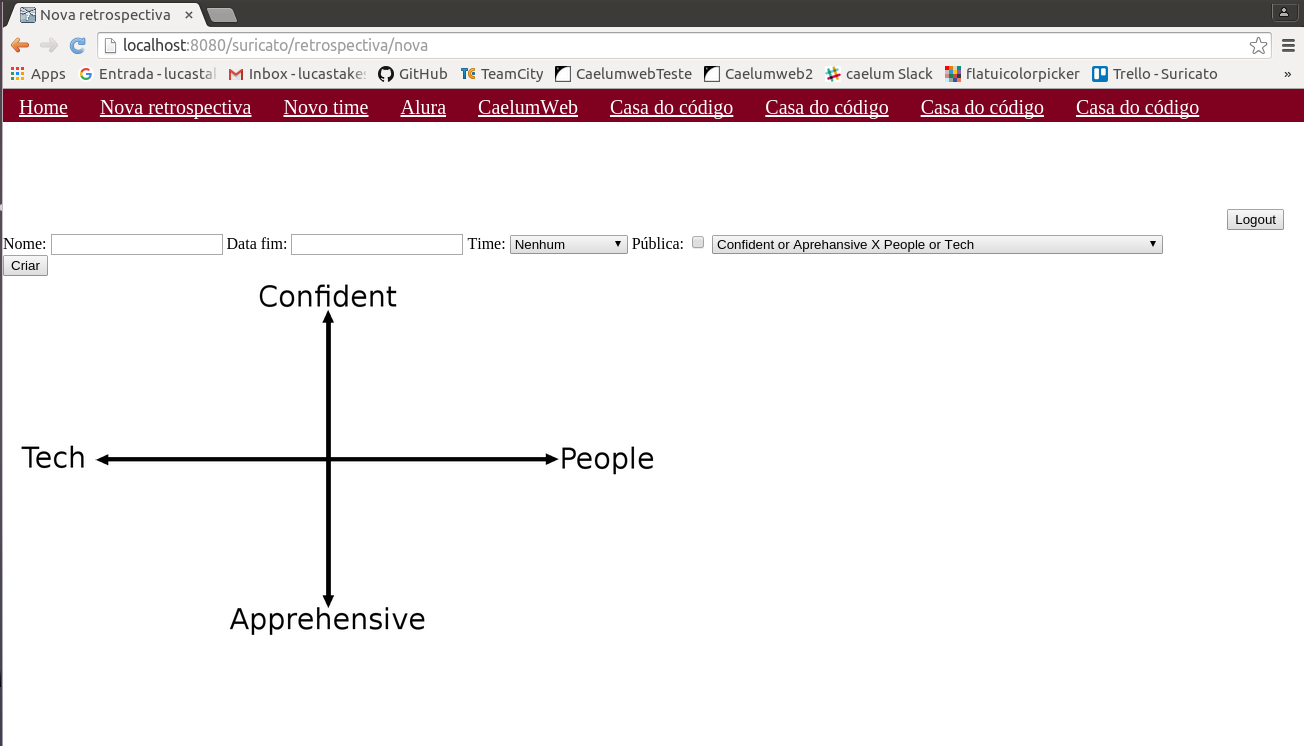
\includegraphics[width=130mm]{images/criar.png}
  }
  \caption{Tela antiga de criar lousa virtual}\label{figura:criarAntigo}
\end{figure}

Antes liberar o sistema para ser usado pelos times era crucial arrumar o layout do sistema. Para isso foi necessário um auxílio de outras pessoas que trabalham na Caelum e tinham mais experiência e poderiam sugerir ideias de como melhorar as páginas do sistema. O designer Fabio Gushiken projetou o logo do sistema inspirado no seu nome. Já o designer Leonardo Guerra desenhou algumas atividades das retrospectivas, como a Speed Car e Hot Air Balloon.

Para melhorar a experiência do usuário, os participantes fizeram uma reunião com o instrutor Marco Bruno, que dá aulas de UX e linguagens Front-End na Caelum. Durante a reunião foi explicado quais eram as funcionalidades do sistema e o estado atual das telas. A partir daí discutimos com o instrutor como remodelar o layout para deixá-lo mais agradável. O desenho do que foi planejado nessa reunião está abaixo.

\begin{figure}[H]
  \centering
  \fbox{
    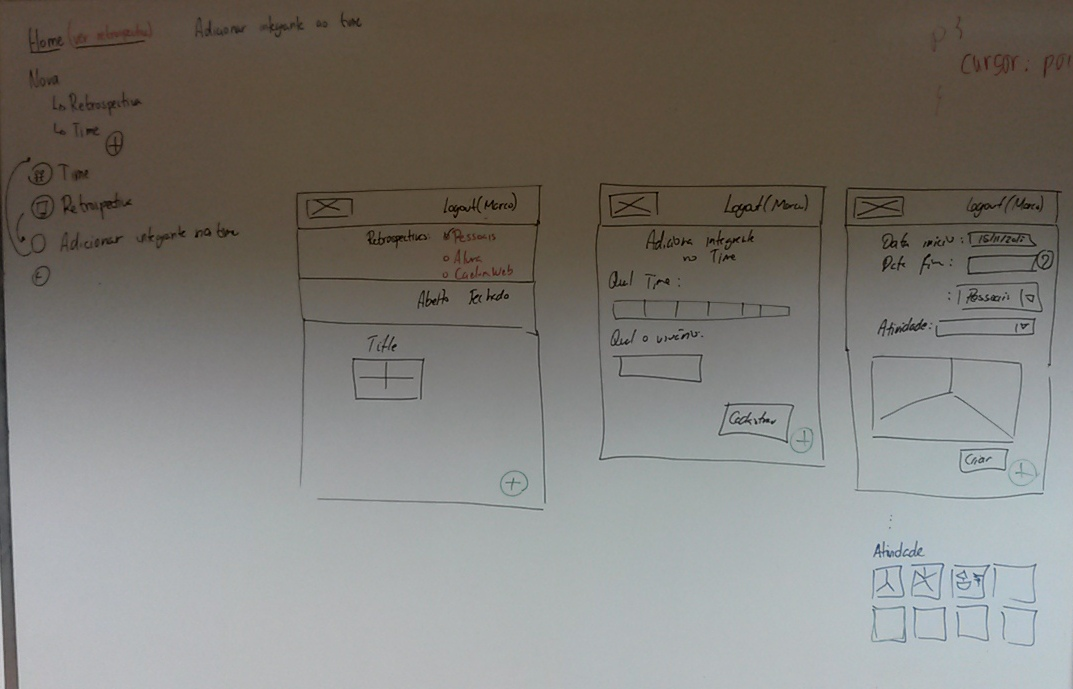
\includegraphics[width=140mm]{images/ux.jpg}
  }
  \caption{Modelagem das telas com UX}\label{figura:ux}
\end{figure}

Portanto, no fim do projeto o foco foi desenvolver as páginas seguindo os que foi planejado na reunião. Atualmente, as telas encontram-se da seguinte forma:

\begin{figure}[H]
  \centering
  \fbox{
    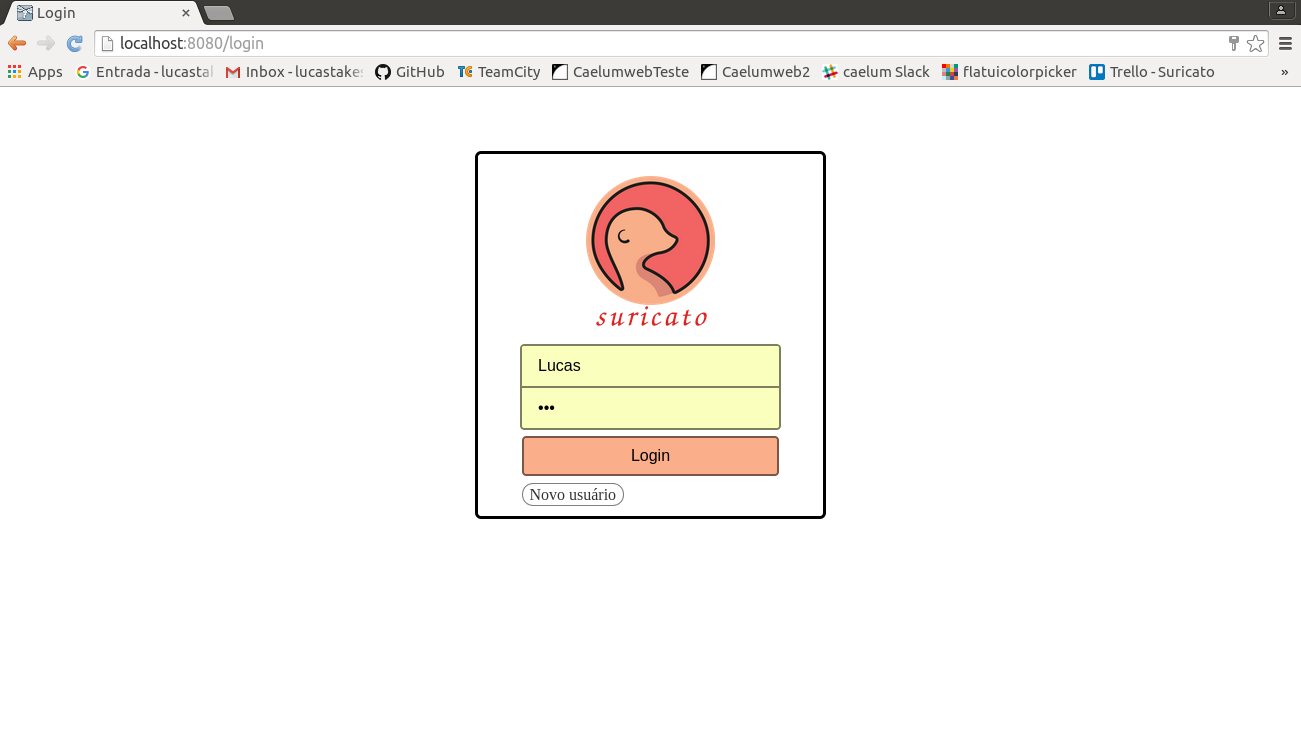
\includegraphics[width=130mm]{images/login2.png}
  }
  \caption{Tela nova de login}\label{figura:loginNovo}
\end{figure}

\begin{figure}[H]
  \centering
  \fbox{
    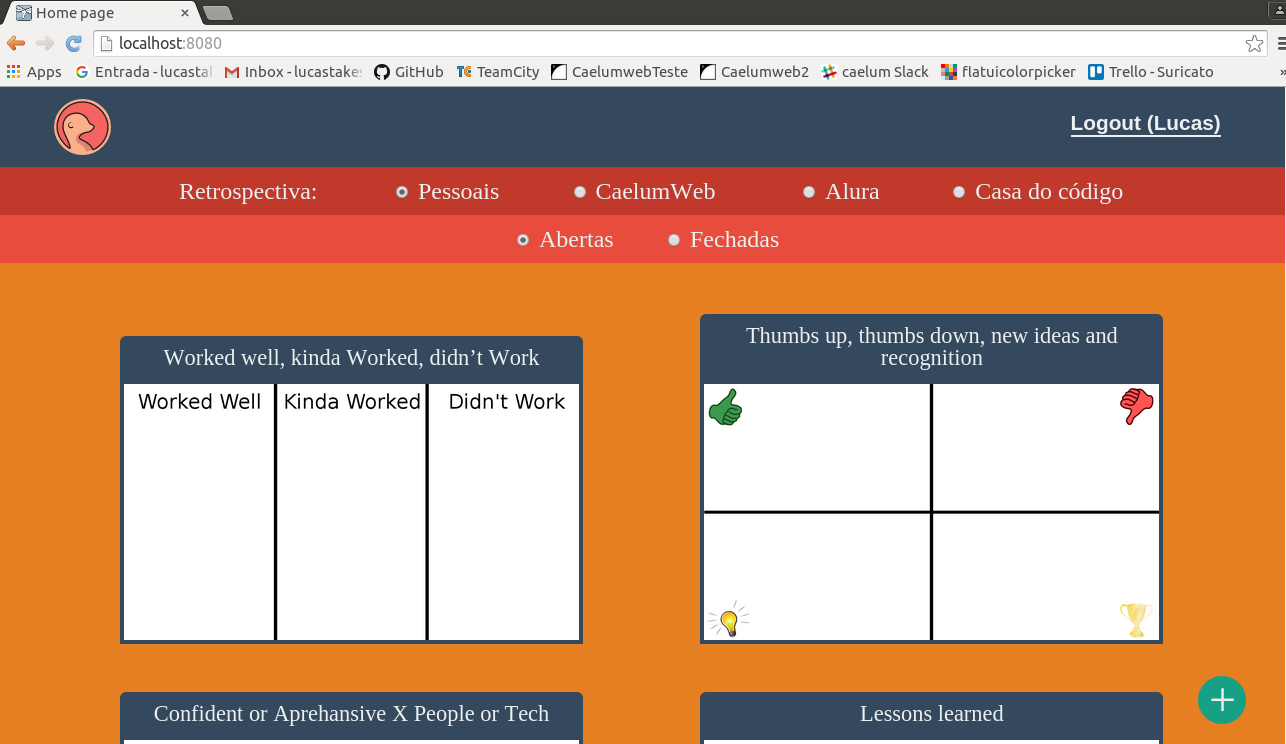
\includegraphics[width=130mm]{images/index2.png}
  }
  \caption{Tela nova do usuário}\label{figura:indexNovo}
\end{figure}

\begin{figure}[H]
  \centering
  \fbox{
    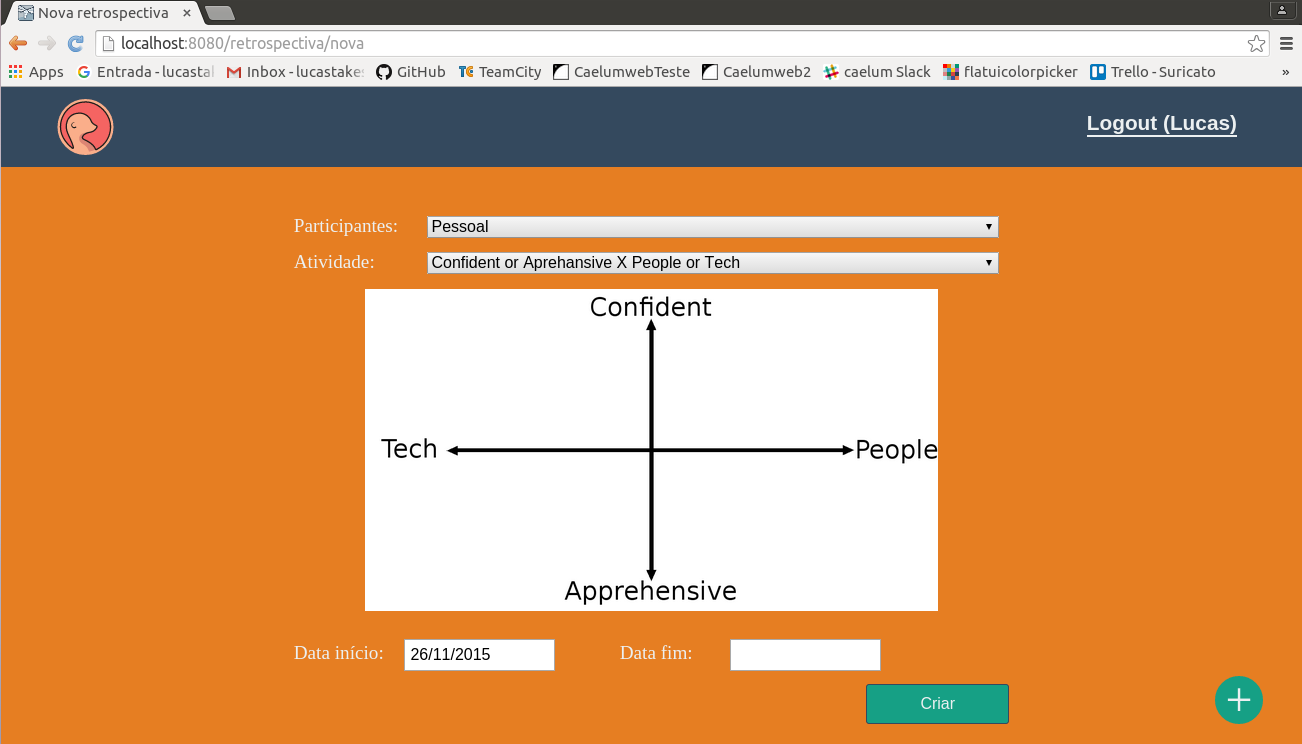
\includegraphics[width=130mm]{images/criar2.png}
  }
  \caption{Tela nova de criar lousa virtual}\label{figura:criarNovo}
\end{figure}

\begin{figure}[H]
  \centering
  \fbox{
    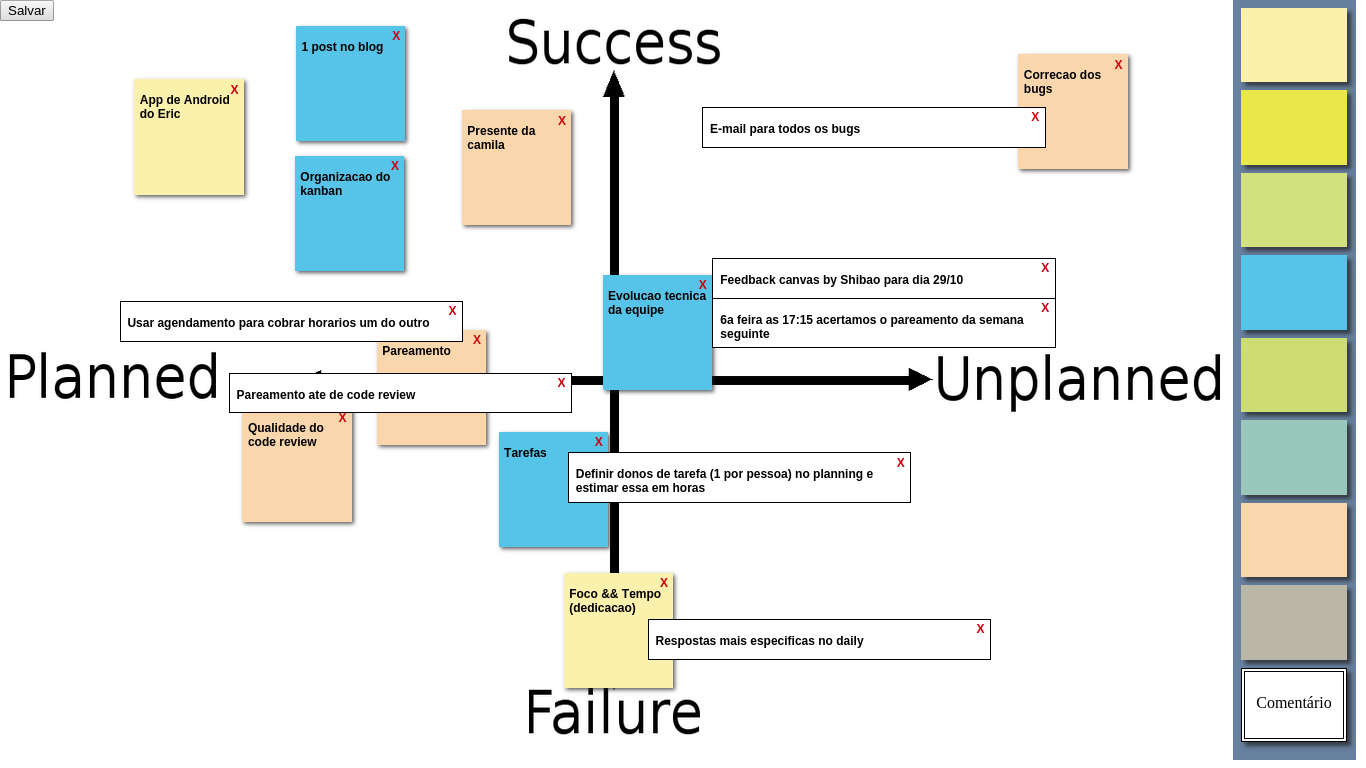
\includegraphics[width=130mm]{images/retrospectiva.png}
  }
  \caption{Tela da lousa virtual}\label{figura:Retrospectiva}
\end{figure}

\subsection{Hospedagem}

Com a primeira versão do sistema pronta, faltava apenas hospedar o site. Como o servidor de aplicação era o WildFly da RedHat, a primeira opção foi usar o serviço da Openshift~\footnote{https://www.openshift.com/}, também da RedHat. Essa plataforma permite que qualquer pessoa hospede de graça sua aplicação web e possui máquinas preparadas para usar o WildFly. Por ser gratuito, o Openshift desliga a máquina quando ninguém está usando o sistema e liga quando um usuário tenta acessá-la. No entanto, para o Suricato as máquinas se mostraram muito instáveis, já que depois de ligá-la o sistema não era colocado no ar automaticamente. Alguém precisava se conectar via ssh na máquina e rodar comandos para que o projeto subisse.

Devido a instabilidade da Openshift, tempos depois o sistema foi hospedado na Amazon Web Services~\footnote{https://aws.amazon.com/}. Mesmo levando alguns dias para criar a máquina e preparar o ambiente para rodar com o WildFly, o serviço é bem mais confiável e estável.

Atualmente o domínio usado para acessar o projeto é http://suricatoagil.com/login.
\newpage

\section{Conclusão}

A ideia inicial do trabalho de desenvolver um aplicação envolvendo diversas tecnologias e seu aprendizado durante o projeto foram plenamente atingidos. Mas, as expectativas iniciais do aprendizado eram menores do que o que foi atingido.

No início do projeto, a proposta do prof. Dr. Alfredo Goldman era uma revisão sistemática sobre retrospectiva. Isto proporcionou uma experiência diferente para a equipe. Através dessa revisão, o conhecimento sobre métodos ágeis e em especial sobre melhoria contínua e retrospectiva tornou-se mais profundo.

A frustração de não encontrar artigos e pesquisas mais detalhados no assunto foi uma situação inesperada. O desenvolvimento de uma pesquisa foi algo novo e desafiador no trabalho. Nenhum dos autores tinha experiência em fazer uma pesquisa acadêmica, o que tornou o processo em um constante aprendizado. Se não fosse a ajuda e influência da Cecília nas comunidades ágeis não seria possível conseguir um conjunto de respostas relevantes.

Outra dificuldade encontrada foi analisar os dados coletados. Os membros não sabiam como interpretar e correlacionar as respostas. A equipe recebeu a ajuda de pessoas da Caelum, em especial ao Mauricio Aniche, e conseguiu encontrar uma forma de analisar os dados, relacionar todas as respostas, e chegar a algumas conclusões. Estas foram vitais na hora de planejar os requisitos da aplicação.

Já havia uma ideia das tecnologias e ferramentas a se utilizar. Os autores já eram familiarizados com Java e Hibernate, então o desafio foi aprender a utilizar e resolver os problemas com as outras tecnologias incorporadas. O principal desafio foi em relação aos WebSockets e SpringSecurity, mas com a ajuda do senhor Alberto Tavares foi possível ajustar toda a configuração do sistema. 

Para o escopo do trabalho o objetivo de colocar a aplicação no ar foi atingido. Como o projeto é \textit{open source}, a equipe agora pode abrir para contribuições externas, já que apenas alguns requisitos foram implementados e ainda há espaço para evoluir.  

O próximo passo do projeto é continuar o desenvolvimento dos requisitos gerados da pesquisa e planejados pela equipe. Por exemplo, um relógio marcando o tempo da reunião, avisos via e-mail e no próprio site sobre as próximas reuniões agendadas, sistema de sugestão de atividades baseado no histórico do time e  usuários criarem novas atividades.

No entanto, o sistema já possui uma quantidade razoável de funcionalidades e consegue ser usado para reuniões de melhoria contínua. Assim, os idealizadores do projeto acreditam que neste momento é mais interessante segurar a implementação de novos recursos e começar a divulgar o sistema para ser usado por mais times além dos presentes na Caelum.

A ideia é primeiro divulgar o sistema para os times que responderam a pesquisa e mandaram o e-mail para contato. Se esses times começarem a utilizar o Suricato é possível refazer a pesquisa e averiguar se o Suricato ajudou no seu processo de melhoria contínua.

Além disso, pretende-se também divulgar o sistema em diversas listas da comunidade ágil e verificar se o Suricato consegue ter uma boa aceitação. Também será disponibilizado no site uma área para as pessoas mandarem sugestões com melhorias que podem ser feitas no sistema ou novas funcionalidades.

Futuramente, ficou planejado realizar uma nova pesquisa buscando responder algumas perguntas que ficaram em aberto, como:

\begin{enumerate}
	\item Times passam pro problemas de falta de engajamento porque não variam os tipos de retrospectiva?
	\item Como exatamente os times distribuídos fazem as suas reuniões de melhoria contínua? Que ferramentas eles utilizam?
	\item A figura do facilitador pode ajudar com algumas das dificuldades encontradas em retrospectivas?
	\item Retrospectiva realmente não tem auxiliado os times com problemas de produtividade? Ou isso ocorre por conta dos times distribuídos serem realmente mais produtivos e terem puxado para  o percentual de times que tem esse problema e que não fazem retrospectiva?
\end{enumerate}

Por fim, caso o Suricato se prove uma ferramenta útil na comunidade, será possível escrever alguns artigos para revistas e submeter palestras em eventos ágeis comentando sobre a ferramenta e os resultados obtidos. 
\newpage

\begin{thebibliography}{7} 

\bibitem{manifesto} Kent Beck, Alistair Cockburn, Martin Fowler, et al. \textit{Agile Manifesto}. http://www.agilemanifesto.org;
\bibitem{retrospectives} Esther Derby, Diana Larsen. \textit{Agile Retrospectives: Making Good Teams Great}. Dallas: The Pragmatic Bookshelf, 2006.
\bibitem{funRetrospectives} Paulo Caroli, Taina Caetano. \textit{Fun Retrospectives: Activities and ideas for making agile retrospectives more engaging}. Leanpub, 2014. https://leanpub.com/funretrospectives
\bibitem{handRetrospectives} Patrick Kua. \textit{The Retrospective Handbook: A guide for agile teams}. Leanpub, 2013. https://leanpub.com/the-retrospective-handbook
\bibitem{lean} Taiichi Ohno, Norman Bodek. \textit{Toyota Production System: Beyond Large-Scale Production}. Productivity Press, 1988. https://books.google.com.br/books?id=7\_-67SshOy8C
\bibitem{versionOne} Version One. \textit{8th Annual State of Agile Survey}. Alpharetta: Version One, 2013. http://www.versionone.com/pdf/2013-state-of-agile-survey.pdf
\bibitem{scrumAlliance} Scrum Alliance. \textit{The 2015 State of Scrum Report}. Westminster: Scrum Alliance, 2015. https://www.scrumalliance.org/why-scrum/state-of-scrum-report/2015-state-of-scrum
\bibitem{poussard} Pascal Poussaard. \textit{Classifying Retrospectives to get the best of it}. 2014. http://www.benlinders.com/2014/guest-blog-classifying-retrospectives-to-get-the-best-of-it

\end{thebibliography}

\newpage

\renewcommand{\appendixname}{Apêndice}
\renewcommand{\appendixpagename}{Apêndices}
\renewcommand{\appendixtocname}{Apêndices}

\appendix
\appendixpage
\addappheadtotoc

\renewcommand\thesection{\Roman{section}}


\section{Questões da pesquisa}
\label{app:resultados}

\textbf{Página 1}
\begin{enumerate}
	\item Como a maioria do seu time é estruturado?
	\begin{enumerate}
		\item Distribuído em time zones diversos
		\item Distribuído no mesmo time zone
		\item Local
	\end{enumerate}
	\item Quais problemas seu time enfrenta? 
	\begin{enumerate}
		\item Comunicação 
		\item Relacionamento 
		\item Produtividade 
		\item Nenhum 
		\item Outros 
	\end{enumerate}
	\item Seu time possui quantos integrantes? 
	\begin{enumerate}
		\item 1 - 10 
		\item 11 - 20 
		\item 21 - 30 
		\item mais de 30 
	\end{enumerate}
	\item Seu time realiza retrospectivas? 
	\begin{enumerate}
		\item Sim 
		\item Não 
	\end{enumerate}
\end{enumerate}

\textbf{Página 2: caso a resposta da pergunta 4 da página 1 seja sim}
\begin{enumerate}
	\item Com que frequência realiza retrospectivas?
	\item Vocês variam as atividades e/ou formato das suas retrospectivas? Se sim, cite alguns.
	\item Quem participa das retrospectivas?
	\item Quais desafios seu time enfrenta ao realizar uma retrospectiva? 
	\begin{enumerate}
		\item Ultrapassar a duração da reunião
		\item Agendar dia, horário e lugar
		\item Discussões de pouco valor 
		\item Falta de intimidade entre os integrantes 
		\item Engajamento das pessoas 
		\item Falta de anonimato 
		\item Outros 
	\end{enumerate}
	\item Vocês utilizam algum site, programa ou ferramenta para ajudar a realizar a retrospectiva? Se sim, cite alguns. 
	\item Alguém fica responsável por ser o facilitador da retrospectiva?
	\begin{enumerate}
		\item Sim 
		\item Não
	\end{enumerate}
\end{enumerate}

\textbf{Página 3: caso a resposta da pergunta 6 da página 2 seja sim}
\begin{enumerate}
	\item O facilitador faz parte do time? Se sim, qual o papel dele no time?
	\begin{enumerate}
		\item Sim
		\item Não
	\end{enumerate}
\end{enumerate}

\textbf{Página 4: caso a resposta da pergunta 4 da página 1 seja não}
\begin{enumerate}
	\item De que forma os problemas que seu time já tem são discutidos e resolvidos? 
	\item De que forma seu time identifica problemas futuros e trabalha para evitá-los? 
	\item Quem participa das discussões sobre os problemas do time? E quem resolve os problemas? 
	\item Quais os motivos para seu time não fazer retrospectivas? 
	\item Com que frequência o time inteiro se reúne, seja local ou virtualmente?
\end{enumerate}

\textbf{Página 5}
\begin{enumerate}
	\item Coloque seu e-mail abaixo, se deseja receber os resultados dessa pesquisa. 
	\item Deseja acrescentar algo sobre seu time, ou deixar algum comentário sobre a pesquisa?
\end{enumerate}
\newpage

\section{Respostas da pesquisa}
\label{respostas}

A pesquisa teve 44 respostas, sendo que 24 pessoas responderam todas as perguntas e 20 apenas a primeira página.

\subsubsection*{Pessoas que responderam apenas a página 1}

\newenvironment{respostas1}[4] {
		\begin{tabular}{| c | m{14em} |}
		\hline
		Como a maioria do seu time é estruturado? & #1 \\
		\hline
		Quais problemas seu time enfrenta?        & #2 \\
		\hline
		Seu time possui quantos integrantes?      & #3 \\
		\hline
		Seu time realiza retrospectivas?          & #4 \\	
		\hline
		\end{tabular}
	
}

\begin{enumerate}
	\item
	\begin{respostas1}
		{Local}
		{Comunicação e relacionamento}
		{1 - 10}
		{Não}
	\end{respostas1}

	\item
	\begin{respostas1}
		{Local}
		{Nenhum}
		{1 - 10}
		{Não}
	\end{respostas1}

	\item
	\begin{respostas1}
		{Local}
		{Nenhum}
		{1 - 10}
		{Sim}
	\end{respostas1}

	\item
	\begin{respostas1}
		{Distribuído no mesmo timezone}
		{Produtividade}
		{1 - 10}
		{Não}
	\end{respostas1}

	\item
	\begin{respostas1}
		{Distribuído no mesmo timezone}
		{Produtividade}
		{21 - 30}
		{Não}
	\end{respostas1}

	\item
	\begin{respostas1}
		{Local}
		{Comunicação}
		{1 - 10}
		{Não}
	\end{respostas1}

	\item
	\begin{respostas1}
		{Local}
		{Comunicação e produtividade}
		{mais de 30}
		{Sim}
	\end{respostas1}

	\item
	\begin{respostas1}
		{Local}
		{Comunicação, relacionamento e produtividade}
		{1 - 10}
		{Não}
	\end{respostas1}

	\item
	\begin{respostas1}
		{Local}
		{Produtividade}
		{1 - 10}
		{Sim}
	\end{respostas1}

	\item
	\begin{respostas1}
		{Local}
		{Comunicação e produtividade}
		{11 -20}
		{Não}
	\end{respostas1}

	\item
	\begin{respostas1}
		{Distribuído no mesmo timezone}
		{Comunicação}
		{1 - 10}
		{Sim}
	\end{respostas1}

	\item
	\begin{respostas1}
		{Distribuído no mesmo timezone}
		{Comunicação}
		{11 - 20}
		{Sim}
	\end{respostas1}

	\item
	\begin{respostas1}
		{Local}
		{Comunicação e produtividade}
		{11 - 20}
		{Não}
	\end{respostas1}

	\item
	\begin{respostas1}
		{Local}
		{Comunicação e produtividade}
		{1 - 10}
		{Sim}
	\end{respostas1}

	\item
	\begin{respostas1}
		{Local}
		{Comunicação}
		{11 - 20}
		{Sim}
	\end{respostas1}

	\item
	\begin{respostas1}
		{Local}
		{Produtividade}
		{1 - 10}
		{Sim}
	\end{respostas1}

	\item
	\begin{respostas1}
		{Local}
		{Comunicação e produtividade}
		{11 - 20}
		{Sim}
	\end{respostas1}

	\item
	\begin{respostas1}
		{Distribuído no mesmo timezone}
		{Produtividade}
		{1 - 10}
		{Sim}
	\end{respostas1}

	\item
	\begin{respostas1}
		{Local}
		{Nenhum}
		{1 - 10}
		{Sim}
	\end{respostas1}

	\item
	\begin{respostas1}
		{Local}
		{Nenhum}
		{1 - 10}
		{Sim}
	\end{respostas1}
\end{enumerate}


\subsubsection*{Respostas completas - times que fazem retrospectiva}

\newenvironment{respostas2}[9] {
		\begin{tabular}{|m{20em}|m{22em}|}
		\hline
		Como a maioria do seu time é estruturado?  & #1 \\
		\hline
		Quais problemas seu time enfrenta?         & #2 \\
		\hline
		Seu time possui quantos integrantes?       & #3 \\
		\hline
		Com que frequência realiza retrospectivas? & #4 \\	
		\hline
		Vocês variam as atividades e/ou formato das suas retrospectivas? Se sim, cite alguns.											& #5 \\
        \hline
		Quem participa das retrospectivas?         & #6 \\
         \hline
		Quais desafios seu time enfrenta ao realizar uma retrospectiva?
												   & #7 \\
        \hline
		Vocês utilizam algum site, programa ou ferramenta para ajudar a realizar a retrospectiva? Se sim, cite alguns.        & #8 \\
        \hline
		Alguém fica responsável por ser o facilitador da retrospectiva?
											       & #9 \\
		\hline
		\end{tabular}
}

\begin{enumerate}[leftmargin=-2em]
	\item
	\begin{respostas2}
		{Local}
		{Produtividade}
		{1 - 10}
		{15 dias}
		{Não}
		{Time de desenvolvimento}
		{Agendar dia, horário e lugar \newline Engajamento das pessoas}
		{Não}
		{Líder técnico}
	\end{respostas2}

	\item
	\begin{respostas2}
		{Local}
		{Comunicação e produtividade}
		{11 - 20}
		{1x a cada 15 dias}
		{Sim. Papel pontos positivos e negativos, reuniões para coversar sem post its,}
		{Todo o time}
		{Discussões de pouco valor \newline Engajamento das pessoas}
		{Não}
		{O facilitador varia, cada retro é uma pessoa}
	\end{respostas2}

	\item
	\begin{respostas2}
		{Local}
		{Nenhum}
		{1 - 10}
		{A cada 2 semanas}
		{Não}
		{Todo o time: scrum master, Dev team e PO}
		{Ultrapassar a duração}
		{Atualmente PO organiza tudo em Excel}
		{Não}
	\end{respostas2}

	\item
	\begin{respostas2}
		{Local}
		{Comunicação, relacionamento e produtividade}
		{1 - 10}
		{A cada 2 semanas}
		{Sim; learning matrix, happiness radar, startfish, etc}
		{Scrum master e time}
		{Discussões de pouco valor \newline Engajamento das pessoas}
		{Não}
		{Sim, mas não é do time}
	\end{respostas2}

	\item
	\begin{respostas2}
		{Local}
		{Outro: Um projeto grande com atividades menores de manutenção de outros projetos. Alternância de foco}
		{1 - 10}
		{A cada 3 semanas}
		{Não}
		{Todo o time de desenvolvimento. Quando é possível tentamos envolver o cliente.}
		{Ultrapassar a duração \newline Engajaento das pessoas}
		{Não}
		{Líder}
	\end{respostas2}

	\item
	\begin{respostas2}
		{Distribuído no mesmo timezone}
		{Comunicação e produtividade \newline Outros: Dependências Não-Gerenciadas}
		{11 - 20}
		{A cada 2 semanas}
		{Sim, variamos! Basicamente elas seguem o formato sugerido pela Esther Derby e Diana Larsen (Agile Retrospectives), mas não linearmente. Utilizo técnicas para: - Criar ambiente seguro para os participantes tocarem em assuntos delicados (working agreements) - Setar o contexto, pedindo que falem um sentimento para a Sprint atual, ou que desenhem como foi a Sprint atual, ou que escrevam em post-its (dependendo do nível de introspectividade do grupo) - Pergunto, em casos de falha, por que a Sprint falhou - Coloco, em casos de sucesso, quais fatores nos fizeram chegar lá, e o que poderíamos fazer para chegarmos lá ainda melhores ou mais cedo - Utilizo um espaço de trabalho informativo, deixando visíveis, board, burndown, meta da Sprint, Definição de Pronto e outros artefatos para iluminar as ideias e trazer possiveis pontos de melhoria - Projeto o burndown maior para fazermos uma timeline em cima dele e dos acontecimentos que ele projeta - Traçamos planos de ação em forma de brainstorming falado ou escrito - Utilizo tecnicas de priorização quando há muitos pontos a serem tratados pelos participantes - Faço o time se apreciar pelo apoio mútuo em atingir a meta - E muitas outras :P}
		{Time, Product Owner, Scrum Master, Agile Coach.Convidados em caso especial, com consentimento dos três acima.}
		{Falta de intimidade entre integrantes \newline Engajamento das pessoas \newline Falta de anonimato}
		{Não}
		{Agile coach ou Scrum master}
	\end{respostas2}

	\item
	\begin{respostas2}
		{Local}
		{Comunicação}
		{1 - 10}
		{A cada fim de sprint (15 dias de interação)}
		{Variamos de acordo com a necessidade. O padrão é fazer um formato de retrospectiva. Mas as vezes temos pouco tempo, ou o sprint teve poucos problemas ai fazemos outro formato. O padrão de fazer a matriz (começar, continuar, melhorar, parar). O formato simples e rápido é colocarmos apenas os assuntos que aconteceram nos post its e ações para melhoras no próximo sprint. Quando o clima esta legal e temos tempo, fazemos outros formatos mais lúdicos, como timeline.}
		{Todos! Po, Time e SM. Ninguém fica de fora para não ter ruido na comunicação e fofoca.}
		{Ultrapassar a duração}
		{Acima já coloquei alguns nos links. Mas como SM sempre tenho o.modelo de PDCA na cabeça. Ou seja, sempre tem que ter melhorias.}
		{Sim, organiza reuniões, facilita conversas, cuida do quadro, auxilia o PO com o Backlog, alinha expectativas com stakeholders, remove impedimentos e acompanha o desenvolvimento individual de cada integrante da equipe!}
	\end{respostas2}

	\item
	\begin{respostas2}
		{Local}
		{Comunicação e produtividade}
		{1 - 10}
		{A cada fim de sprint (2 semanas)}
		{Sim, dependendo do que queremos mostrar.; Team building com this guy/that guy, timelines e do's and don'ts, starfish, (stop/start/continue), dinamicas de apreciação, etc. sempre atendo-se ao formato de "warm-up, coleta de dados, discussão e ações". para cada ação que levantamos, colocamos um dono dela, que será responsável por fazê-la acontecer}
		{Apenas os membros do time}
		{Discussão de pouco valor \newline Engajamento das pessoas}
		{Não}
		{Sim}
	\end{respostas2}

	\item
	\begin{respostas2}
		{Local}
		{Comunicação e produtividade \newline Outros: capacitação}
		{1 - 10}
		{A cada sprint}
		{Não}
		{Todo o time, mais um integrante de uma equipe separada responsável por Qualidade de Processos (uma espécie de "escritório" de SMs).}
		{Ultrapassar a duração \newline Discussão de pouco valor \newline Falta de intimidade integrantes \newline Engajamento das pessoas}
		{Um quadro. Pra organizar os itens que foram bons, os que precisam melhorar e as ações de melhoria.}
		{Scrum master}
	\end{respostas2}

	\item
	\begin{respostas2}
		{Local}
		{Produtividade}
		{1 - 10}
		{Ao final de cada sprint}
		{Não}
		{Scrum Team}
		{Engajamento das pessoas \newline Outro: Olham como obrigação e não como um momento para a melhoria do processo.}
		{Não}
		{Scrum master}
	\end{respostas2}

	\item
	\begin{respostas2}
		{Local}
		{Comunicação, relacionamento e produtividade}
		{1 - 10}
		{Fim de projeto}
		{Não}
		{Todo time}
		{Ultrapassar a duração}
		{Não}
		{Sim, mas não é do time}
	\end{respostas2}

	\item
	\begin{respostas2}
		{Distribuído em diversos timezones}
		{Comunicação}
		{21 - 30}
		{Final de cada sprint}
		{Não}
		{O time, PO e Gps}
		{Discussão de pouco valor}
		{Não}
		{Sim, o gp}
	\end{respostas2}

	\item
	\begin{respostas2}
		{Distribuído no mesmo timezone}
		{Nenhum}
		{11 - 20}
		{Mensal}
		{Não}
		{Todo o time}
		{Ultrapassar a duração \newline Discussões de pouco valor \newline Falta de intimidade entre integrantes}
		{Não}
		{PO}
	\end{respostas2}

	\item
	\begin{respostas2}
		{Distribuído no mesmo timezone}
		{Comunicação e relacionamento}
		{1 - 10}
		{Postmortem}
		{Não}
		{Todos os integrantes do time}
		{Discussões de pouco valor \newline Falta de intimidade entre entegrantes}
		{Não}
		{Líder ou gerente}
	\end{respostas2}

	\item
	\begin{respostas2}
		{Local}
		{Produtividade}
		{1 - 10}
		{Quinzenal}
		{Sim. Usamos algumas técnicas: fishbowl, morte do produto, brainstorm, brainstorm reverso, hot-air ballon, 6 chapéus e outros.}
		{Time, Scrum Master e PO}
		{Ultrapassar a duração}
		{Fun retrospectives}
		{Scrum master ou Dev}
	\end{respostas2}

	\item
	\begin{respostas2}
		{Distribuído no mesmo timezone}
		{Nenhum}
		{1 - 10}
		{Quinzenal}
		{Sim}
		{Todos do time, PO, Devs, tester, suporte.}
		{Ultrapassar a duração \newline Outro: perder o foco}
		{Não}
		{Revesado, todos um dia é facilitador.}
	\end{respostas2}

	\item
	\begin{respostas2}
		{Distribuído no mesmo timezone}
		{Comunicação}
		{11 - 20}
		{Semanalmente}
		{Discutimos o que está ruim e precisamos mudar, o que foi bom e precisamos continuar. Além disso sempre discutimos alguns assuntos que necessitam da presença de todos.; Vez por outra fazemos algumas práticas como: o Fishbowl.}
		{Ao total dura entre 1h e 1:30h. Temos 2 times: operações e desenvolvimento. nos primeiros 30min cada time faz sua própria retro para alinhamento de quesitos que compete somente a cada time. Depois os times se reúnem e abordam questões que envolvem os dois times.}
		{Ultrapassar a duração \newline Outro: Por vezes é necessário alguém da diretoria na reunião. O que acontece de vez enquando.}
		{Utilizamos apenas o quadro branco. Quando é necessário usamos folhas e canetas para anotações ....}
		{É aleatório ... lidera quem quer sempre respeitando para não ser sempre o mesmo}
	\end{respostas2}

	\item
	\begin{respostas2}
		{Local}
		{Produtividade}
		{1 - 10}
		{Sempre}
		{Não}
		{Dev, PO e SM}
		{Ultrapassar a duração}
		{Não}
		{Não}
	\end{respostas2}

	\item
	\begin{respostas2}
		{Local}
		{Produtividade}
		{1 - 10}
		{Todo sprint, que tem duração de 4 semanas}
		{Não}
		{somente time de desenvolvimento}
		{Discussão de pouco valor \newline Falta de engajamento}
		{Não}
		{Scrum master}
	\end{respostas2}
\end{enumerate}

\subsubsection*{Respostas completas - times que não fazem retrospectiva}

\newenvironment{respostas3}[8] {
		\begin{tabular}{|m{18em}|m{18em}|}
		\hline
		Como a maioria do seu time é estruturado?  & #1 \\
		\hline
		Quais problemas seu time enfrenta?         & #2 \\
		\hline
		Seu time possui quantos integrantes?       & #3 \\
		\hline
		De que forma os problemas que seu time já tem são discutidos e resolvidos? 
												   & #4 \\	
		\hline
		De que forma seu time identifica problemas futuros e trabalha para evitá-los? 												   & #5 \\
        \hline
		Quem participa das discussões sobre os problemas do time? E quem resolve os problemas? 							       & #6 \\
         \hline
		Quais os motivos para seu time não fazer retrospectivas? 
												   & #7 \\
        \hline
		Com que frequência o time inteiro se reúne, seja local ou virtualmente? 
											       & #8 \\
		\hline
		\end{tabular}
}

\begin{enumerate}[leftmargin=0.5em]
	\item
	\begin{respostas3}
		{Distribuído em timezones diversos}
		{Comunicação e produtividade}
		{11 - 20}
		{Chat direto entre a pessoa que está problema e a pessoa que pode resolve-lo.}
		{Não há um meio formal para tal. Temos chats no Skype que usamos pra discutir dúvidas, soluções, sugestões, etc. Cada sub-time (front, back, db) possui um chat, e um chat entre os "cabeças" de cada sub-time, e um chat com o time todo. São criados chats sob demanda também.}
		{Não há alguém encarregado, normalmente todas as opiniões são escutadas e discutidas, e tentamos seguir a melhor solução.}
		{Má gerência. Nosso gerente é muito inexperiente com essas metodologias. De pouco em pouco estamos corrigindo isso.}
		{Todos os dias, via chat.}
	\end{respostas3}

	\item
	\begin{respostas3}
		{Distribuído em timezones diversos}
		{Comunicação \newline Outros: sincronização}
		{11 - 20}
		{Conference as por telefone ou online}
		{Falhadas Rapido Melhor do que falhar tarde, assim mais facil identificar o problema em algo}
		{Todos is envolvidos. Depende da complex idled e importancia fermented Sao envolvidos}
		{Sem motivos aparentes, Altas quabtidades de demandas para time restrito em quantidade de recursos}
		{cada celula tem reunions diarias de sync e o time inteiro se reune a Casa Laguna meses}
	\end{respostas3}

	\item
	\begin{respostas3}
		{Distribuído em timezones diversos}
		{Relacionamento \newline Outros: Equipes descentralizadas e pouco integradas}
		{Mais de 30}
		{Reuniões informações e sem hora prevista}
		{Por demanada.}
		{Líderes de projetos junto com a equipe.}
		{Atualmente os prazos estão comprometidos junto aos cliente (entregas). Por isso temos tido pouco tempo para executar reunioes de verificação.}
		{Quase nunca. Muita gente}
	\end{respostas3}

	\item
	\begin{respostas3}
		{Distribuído em timezones diversos}
		{Relacionamento}
		{Mais de 30}
		{Em reuniões com os integrantes envolvidos no problema, caso o problema seja de utilidade para todo o time, a solução é repassada posteriormente ao time todo.}
		{De uma forma geral, não há esse tipo de preocupação.}
		{Quem está envolvido no problema e os responsáveis pelo produto, como product owner, analistas, diretores, etc.}
		{Não sei exatamente, decisão dos gestores do projeto.}
		{Diariamente.}
	\end{respostas3}

	\item
	\begin{respostas3}
		{Distribuído em timezones diversos}
		{Comnicação \newline Outros: Agilidade para corrigir bug ou entrar novas funcionalidades quando para concluir a tarefa precisa do envolvimento de outros membros da equipe}
		{1 - 10}
		{Muitas das vezes tentamos realizar um call com todos os membros de forma que o timezone fica fácil para todos. Quando identificamos os problemas cada um da sua opinião de como podemos melhorar a situação e o Gerente de Projetos se encarrega de seguir a opinião que decidimos.}
		{O time é muito focado na parte do código, então quando achamos que pode acontecer algum problema em certo ponto da aplicação, colocamos um alerta nesse ponto para que o time olhe e decida qual o melhor caminho para realizar.}
		{Todos os membros da equipe, normalmente fica a cargo do gerente de projetos e líder de equipe}
		{Não é uma cultura da empresa, nem da equipe. Acaba não dando atenção neste aspecto.}
		{3 - 4 vezes por mês}
	\end{respostas3}
\end{enumerate}
\newpage

\end{document}
